% Definiciones y constantes de estilo
% Clase del documento
\documentclass[a4paper,12pt,twoside,openright,titlepage]{book}

%
% Paquetes necesarios
%
\usepackage[T1]{fontenc}
\usepackage{pslatex}
% Símbolo del euro
\usepackage{eurosym}
% Codificación UTF8
\usepackage[utf8]{inputenc}
% Caracteres del español
\usepackage[spanish]{babel}
% Código, algoritmos, etc.
\usepackage{listings}
% Definición de colores
\usepackage{color}
% Extensión del paquete color
\usepackage[table,xcdraw]{xcolor}
% Márgenes
\usepackage{anysize}
% Cabecera y pie de página
\usepackage{fancyhdr}
% Estilo título tulos
\usepackage{quotchap}
% Algoritmos (expresarlos mejor)
\usepackage{algorithmic}
% Títulos de secciones
\usepackage{titlesec}
% Fórmulas matemáticas
\usepackage[cmex10]{amsmath}
% Enumeraciones
\usepackage{enumerate}
% Páginas en blanco
\usepackage{emptypage}
% Separación entre cajas
\usepackage{float}
% Imágenes
\usepackage[pdftex]{graphicx}
% Mejora de las tablas

\usepackage{array}
% Mejora de los símbolos matemáticos
\usepackage{mdwmath}
% Separar figuras en subfiguras
\usepackage[caption=false,font=footnotesize]{subfig}
% Incluir pdfs externos
\usepackage{pdfpages}
% Mejoras sobre las cajas
\usepackage{fancybox}
% Apéndices
\usepackage{appendix}
% Marcadores (para el pdf)
\usepackage{bookmark}
% Estilo de enumeraciones
\usepackage{enumitem}
% Espacio entre líneas y párrafos
\usepackage{setspace}
% Glosario/Acrónimos
\usepackage[acronym]{glossaries}
% Fuentes
\usepackage[T1]{fontenc}
% Bibliografía
\usepackage[sorting=none,natbib=true,backend=bibtex,bibencoding=ascii]{biblatex}
% Fix biblatex+babel warning
\usepackage{csquotes}
\usepackage{afterpage}
%Poner margenes al documento
\usepackage[centering, margin={2.54cm,2.54cm}, includeheadfoot]{geometry}




% Enlaces
\hypersetup{hidelinks,pageanchor=true,colorlinks,citecolor=Fuchsia,urlcolor=black,linkcolor=Cerulean}

%Capacidades matemáticas extra
\usepackage{amsmath} 
%librería de símbolos
\usepackage{amssymb}

% Euro (€)
\DeclareUnicodeCharacter{20AC}{\euro}

% Inclusión de gráficos
\graphicspath{{./graphics/}}

% Texto referencias
\addto{\captionsspanish}{\renewcommand{\bibname}{Bibliografía}}

% Extensiones de gráficos
\DeclareGraphicsExtensions{.pdf,.jpeg,.jpg,.png}

% Definiciones de colores (para hidelinks)
\definecolor{LightCyan}{rgb}{0,0,0}
\definecolor{Cerulean}{rgb}{0,0,0}
\definecolor{Fuchsia}{rgb}{0,0,0}

% Keywords (español e inglés)
\def\keywordsEn{\vspace{.5em}
{\textbf{\textit{Key words ---}}\,\relax%
}}
\def\endkeywordsEn{\par}

\def\keywordsEs{\vspace{.5em}
{\textbf{\textit{Palabras clave ---}}\,\relax%
}}
\def\endkeywordsEs{\par}


% Abstract (español e inglés)
\def\abstractEs{\vspace{.5em}
{\textbf{\textit{Resumen ---}}\,\relax%
}}
\def\endabstractEs{\par}

\def\abstractEn{\vspace{.5em}
{\textbf{\textit{Abstract ---}}\,\relax%
}}
\def\endabstractEn{\par}

% Estilo páginas de capítulos
\fancypagestyle{plain}{
\fancyhf{}
\fancyfoot[CO]{\footnotesize\emph{\nombretrabajo}}
\fancyfoot[RO]{\vspace{0.4cm}\thepage}
\renewcommand{\footrulewidth}{.6pt}
\renewcommand{\headrulewidth}{0.0pt}
}

% Estilo resto de páginas
\pagestyle{fancy}

% Estilo páginas impares
\fancyfoot[CO]{\footnotesize\emph{\nombretrabajo}}
\fancyfoot[RO]{\vspace{0.4cm}\thepage}
%\fancyfoot[LO]{
\includegraphics[width=.08\textwidth]{escudo}}

\rhead[]{\leftmark}


% Estilo páginas pares
\fancyfoot[CE]{\emph{\pieparcen}}
\fancyfoot[LE]{\vspace{0.4cm}\thepage}
%\fancyfoot[RE]{
\includegraphics[width=.08\textwidth]{escudo}}
\lhead[\leftmark]{}


% Guía del pie de página
\renewcommand{\footrulewidth}{.6pt}

% Nombre de los bloques de código
\renewcommand{\lstlistingname}{Código}

% Estilo de los lstlistings
\lstset{
    frame=tb,
    breaklines=true,
    postbreak=\raisebox{0ex}[0ex][0ex]{\ensuremath{\color{gray}\hookrightarrow\space}}
}

% Definiciones de funciones para los títulos
\newlength\salto
\setlength{\salto}{3.5ex plus 1ex minus .2ex}
\newlength\resalto
\setlength{\resalto}{2.3ex plus.2ex}

% Estilo de los acrónimos
\renewcommand{\acronymname}{Glosario}
\renewcommand{\glossaryname}{Glosario}
\pretolerance=2000
\tolerance=3000

% Texto índice de tablas
\addto\captionsspanish{
\def\tablename{Tabla}
\def\listtablename{\'Indice de tablas}
}

% Traducir appendix/appendices
\renewcommand\appendixtocname{Anexos}
\renewcommand\appendixpagename{Anexos}

% Comando code (lstlisting sin cambio de página)
\lstnewenvironment{code}[1][]%
  { \noindent\minipage{0.935\linewidth}\medskip
    \vspace{5mm}
    \lstset{basicstyle=\ttfamily\footnotesize,#1}}
  {\endminipage}
  
% Colores

\definecolor{rositaoscuro}{RGB}{219, 0, 122}


% Definiciones de comandos
\newcommand{\nombreautor}{Miriam Rubio Lecuona}
\newcommand{\nombretutor}{Marisol Gómez Fernández, Alicia Martínez Ramírez}
\newcommand{\nombretrabajo}{Evaluación del movimiento de las manos mediante el uso de fibras de Bragg y sensores inerciales}
\newcommand{\fecha}{Junio de 2019}
\newcommand{\grado}{TODO: Grado}
% Descomentar si tu trabajo tiene un ponente
%\newcommand{\nombreponente}{TODO: Nombre del ponente}
% Descomentar si tu trabajo está asociado a un grupo de investigación
%\newcommand{\grupoInvestigacion}{TODO: Grupo de investigación}
\newcommand{\departamento}{Departamento de Matemáticas}

\newcommand{\universidad}{Universidad Pública de Navarra}
\newcommand{\pieparizq}{TODO: Pie de página par}
\newcommand{\pieparcen}{Trabajo de Fin de Máster}
\newcommand{\logo}{Logo_Upna}
\newcommand\blankpage{%
	\null
	\thispagestyle{empty}%
	\addtocounter{page}{-1}%
	\newpage}

% Glosario y acrónimos
\makeglossaries
% Acrónimos

% TODO: Añadir aquí los acrónimos
% Ejemplo de acrónimo
\newacronym{FPGA}{FPGA}{Field-Programmable Gate Array}

% Glosario

% TODO: Añadir aquí las definiciones del glosario
% Ejemplo de glosario
\newglossaryentry{bitstream}{name={bitstream},description={En este contexto se refiere al binario que configura el Hardware de la FPGA}}

% Rerefencias
\bibliography{src/bibliografia}

% Inicio del documento
\begin{document}

% Elección del idioma (español)
\selectlanguage{spanish}

%
% Portada
%
\pagenumbering{gobble}
%
% Portada
%


\includepdf{cover.pdf}
% Primera página
\pagenumbering{Alph}
\thispagestyle{empty}

\begin{flushleft}
	\begin{scriptsize}
	\end{scriptsize}\end{flushleft}

	\thispagestyle{empty}
	\begin{center}
		
		% Nombre del trabajo
		\textbf{\begin{large}
				\MakeUppercase{\nombretrabajo}\\*
			\end{large}}
			\vspace*{2cm}
			\begin{figure}[H]
				\centering
				
\includegraphics[]{escudo}
			
			\end{figure}
			\vspace{3cm}
			
			% Nombre del autor y del tutor
			\large Autora: \nombreautor \\*
			\large Tutoras: \nombretutor \\*
			\vspace*{1.5cm}
					
			\departamento \\
%			\facultad \\
			\universidad \\
			\vspace{1cm}
			\fecha \\
			
			\clearpage
			
		\end{center}
		\normalsize

\hypersetup{pageanchor=true}

% Estilo de párrafo de los capítulos
\setlength{\parskip}{0.75em}
\renewcommand{\baselinestretch}{1.25}
% Interlineado simple
\spacing{1.5}

%
% Agradecimientos
%
\pagenumbering{Roman}
\setcounter{page}{0}
\chapter*{Agradecimientos}

Escribir agradecimientos  

%
% Resumen
%
% Resumen en inglés
\chapter*{Resumen}

\begin{abstractEn} 
Human gait analysis is commonly used in rehabilitation, sport training and functional diagnosis. Ambulatory systems for assessing human movements must be portable, ergonomic and economically viable. 

The main aim of this work is to design an ultrasound based wireless measuring system to calculate step distances during walking.

The low-cost ultrasonic sensor developed allows us to calculate step distances. The distance has been achieved by merging data provided by our measurement system and by commercial inertial sensors. To ensure the best performance of the system, the accuracy of the ultrasonic sensor has been estimated.

Our results will be very useful in areas such as neurorehabilitation as they provide objective measurements of the rehabilitation and improvement degree in patients with stroke.



\end{abstractEn}

% Palabras clave en inglés
\begin{keywordsEn}
Inertial sensor, Ultrasonic sensor, Step distance measurement, Stroke.
\end{keywordsEn}

% Resumen en español
\chapter*{Resumen}

\begin{abstractEs}
 El análisis de la marcha es habitual en áreas como rehabilitación, entrenamiento deportivo y diagnóstico funcional. Los sistemas de medida ambulatorios deben ser portátiles, ergonómicos y de bajo coste.
 
 El objetivo principal de este trabajo es el diseño de un sistema de medida basado en la tecnología de ultrasonido para calcular la distancia de separación entre pasos durante la marcha.
 
 El sensor de ultrasonido desarrollado permite calcular dicha distancia combinando los datos del sensor de ultrasonido con los proporcionados por sensores inerciales comerciales. Para asegurar el correcto funcionamiento del sistema se ha evaluado la precisión del sensor de ultrasonidos diseñado.
 
 Los resultados serán de gran utilidad en el campo de la neuro-rehabilitación debido a que permiten obtener datos objetivos sobre el grado de mejora en pacientes que han sufrido un ictus.



\end{abstractEs}

% Palabras clave en español
\begin{keywordsEs}
Sensor inercial, Sensor ultrasonido, Distancia de paso, Ictus.
\end{keywordsEs}


%
% Glosario
%
%\printglossary[title=Glosario,toctitle=Glosario]
%\printglossary[title=Acrónimos,toctitle=Acrónimos,type=\acronymtype]

% Estilo de párrafo de los índices
\setlength{\parskip}{1pt}
\renewcommand{\baselinestretch}{1}

%
% Tabla de contenidos
%
\tableofcontents
\afterpage{\blankpage}
\listoftables

\listoffigures


% Estilo de párrafo de los capítulos
\setlength{\parskip}{0.75em}
\renewcommand{\baselinestretch}{1.25}
% Interlineado simple
\spacing{1.5}
% Numeración contenido
\pagenumbering{arabic}
\setcounter{page}{1}



%
% Introducción
%

\chapter{Introducción}

asdf

Introducimos un poco, con algún dato relevante la capacidad de medir el movimiento de las manos. 
O la bondad de esta capacidad aplicándola en rehabilitación.


\section{Justificación}
\label{sec:justificacion1}

\section{Planteamiento del problema}
\label{sec:planteamiento1}

\section{Objetivos}
\label{sec:objetivos1}
Se pretende realizar...

\subsection{Objetivo principal}
\label{sec:objPrinc1}

\subsection{Objetivos específicos}
\label{sec:objEspec1}


\section{Descripción de los apartados del trabajo}
\label{sec:disposicion1}

estructura del documento...

\textbf{Desarrollo del proyecto}
Para la realización de este trabajo se han tomado dos de las tecnologías expuestas en el capítulo \ref{sec:estado_del_arte} y se han llevado a la práctica. De esta manera se puede trabajar empíricamente con dos tecnologías diferentes planteadas como solución para un mismo problema. Una vez realizado todo el trabajo experimental se puede proceder a evaluar las características prácticas de cada tecnología y compararlas entre ellas. 

En función de la tecnología en que la se apoya cada uno de las soluciones, %por un lado se estudian los sensores de fibra FBG, capítulo \ref{sec:FBG3}, y por otro lado, los sensores IMU, capítulo \ref{sec:IMU3}.  
este capítulo se estructura de la siguiente manera: 
\begin{itemize}
	\item {\textbf{\ref{sec:FBG3}}    .- Solución con sensores de fibra FBG} 
	\item {\textbf{\ref{sec:IMU3}}    .- Solución con sensores IMU}
\end{itemize}
Dentro de cada punto se detalla toda la información necesaria para la implementación de cada uno de los sistemas. En ambos casos, la exposición de la solución tomada se divide en la explicación teórica en el \textit{Marco conceptual} y el ensayo práctico en el \textit{Desarrollo del prototipo}. El desarrollo del prototipo estudia los materiales empleados, el proceso de fabricación y el funcionamiento. 



\section{---------------}

---------------------------------------------------------------

Según datos del Grupo de Estudio de Enfermedades Cerebrovasculares de la Sociedad Española de Neurología, el ictus es la primera causa de mortalidad entre las mujeres españolas y la segunda en hombres \cite{ictuss}. jrjr

Se conoce como ictus al conjunto de enfermedades que afectan a los vasos sanguíneos encargados de suministrar la sangre al cerebro. Este grupo de patologías, conocidas popularmente como embolias, también se denominan accidentes cerebrovasculares (ACV) y se manifiestan súbitamente. Según la causa del accidente cerebrovascular, pueden clasificarse en dos tipos: los hemorrágicos (o hemorragias cerebrales) y los isquémicos (o infartos cerebrales). Los ictus hemorrágicos se producen cuando un vaso sanguíneo se rompe y los ictus isquémicos ocurren cuando una arteria se obstruye por la presencia de un coágulo de sangre que a menudo se origina en el corazón y se desplaza hasta el cerebro interrumpiendo el flujo sanguíneo. Tras un ictus, el daño cerebral adquirido puede ser irreparable y dejar secuelas graves que repercutan de forma notable en la calidad de vida de los afectados \cite{ictus_def}.

Las secuelas que sufren los pacientes tras padecer un ictus se reflejan en múltiples aspectos como \cite{secuelas} :
\begin{itemize}
	\item Secuelas y complicaciones físicas: hemiplejia, hemiparesia...
	\item Alteraciones del humor: depresión.
	\item Alteraciones cognitivas: percepción, memoria y atención.
	\item Alteraciones para las actividades de la vida diaria.
\end{itemize}

Para poder lograr minimizar las discapacidades que experimentan estos pacientes al sufrir un ictus y poder así facilitar la integración social de estas personas, la rehabilitación juega un papel fundamental. Una de las funciones que se intenta recuperar con dicha rehabilitación es la marcha ya que en el 80 \% de los casos se ve limitada. Por ello, disponer de sistemas de medida que permitan obtener datos objetivos de parámetros relativos a la marcha permite una caracterización más detallada de la misma. Así, el personal sanitario encargado de su rehabilitación podrá implementar protocolos clínicos más efectivos y personalizados a cada paciente. Además, el poder optimizar la rehabilitación permite un ahorro en el gasto sanitario el cual supone entre un 7 \% y 10 \% en el caso de España \cite{gasto}.

Para determinar de la evolución de la rehabilitación de la marcha uno de los parámetros considerados relevantes es el de la distancia de separación entre pasos. Conociendo dicho dato se puede obtener una valoración objetiva de la estabilidad y ajustar la rehabilitación a las condiciones del paciente.

Dado que el traslado de pacientes con movilidad reducida a laboratorios de biomecánica es costoso y complicado \cite{gasto}, diseñar sistemas de medida portables y de alta precisión supone un gran reto. Estos sistemas permitirían realizar una rehabilitación más personalizada, y por tanto, más eficaz, ,mejorando la calidad de vida de los pacientes y también reducir la inversión que estas personas necesitan





\section{Objetivo}\label{sec:objetivos}
Se pretende realizar el diseño de un sistema inalámbrico de medida que permita obtener datos de la distancia entre pasos en pacientes de neuro-rehabilitación que han sufrido un ictus. El objetivo final es obtener una valoración objetiva de la evolución de su recuperación.

En su diseño, se tendrá en cuenta: La ergonomía del mismo, la autonomía y el coste. Asimismo deberá cumplir con unas especificaciones de resolución óptimas para poder obtener datos fiables.


\section{Estructura del documento}

El documento consta de los siguientes capítulos: 

\begin{itemize}
	\item {CAPÍTULO 1: Introducción.}
	\item {CAPÍTULO 2: Estado del arte.}
	\item {CAPÍTULO 3: Metodología.}
	\item {CAPÍTULO 4: Resultados.}
	\item {CAPÍTULO 5: Conclusiones.}
\end{itemize}



\thispagestyle{empty}
% Estado del arte
%
\chapter{Estado del Arte\label{sec:estado_del_arte}}

[Quizá convenga en este apartado comenzar enfocando el problema a la captación del movimiento en general y despues pasar, al tema de la rehabilitación de manos]

Dada la importancia de la capacidad de capturar el movimiento de las manos cada vez son más los proyectos basados en este eje central.\\
-esto no encaja bien aquí  \\
Desde el estudio de la manera de estudiar el movimiento de cualquier parte del cuerpo de los humanos, hasta el estudio del movimiento de elementos creados por el ser humano. \\ %salto de línea.



\section{Tecnologías para la medida del movimiento}
\label{sec:tecnologias2}

Tecnologías capaces de medir el movimiento...


En la actualidad existen diferentes sistemas que permiten medir el movimiento. En este capítulo se van a explicar brevemente varios de esos sistemas existentes.En este capítulo se detalla el estudio realizado sobre estos sistemas.


Las tecnologías capaces de medir el movimiento a exponer en el capítulo son:
\begin{itemize}
	\item {Cámaras}
	\item {Fibras FBG}
	\item {IMU}
	\item {Sensores capacitivos}
	\item {Sensores mioeléctricos}
\end{itemize}

En este trabajo se estudian más en profundidad las fibras FBG y los sensores IMU. Para ello se han desarrollado dos prototipos, uno basado en las fibras de Bragg y el segundo en los sensores IMU.

\subsection{Cámaras}
\label{sec:camaras2}
asdf

\subsection{FBG}
\label{sec:fbg2}
asdf

\subsection{IMU}
\label{sec:imu2}
asdf

\subsection{Sensores capacitivos}
\label{sec:capacitivos2}
asdf

\subsection{Sensores mioeléctricos}
\label{sec:mioelectricos2}
asdf


\section{Rehabilitación de las manos}
\label{sec:Rehabilitacion2}
Puesto que este trabajo se ha realizado enfocado hacia la actividad de rehabilitación de las manos es conveniente dedicar un espacio a la explicación de las aplicaciones de este tipo de rehabilitación.\\
\subsection{Fundamentos de las manos}
\label{sec:manos2}
Exponer un poco como es la fisionomía de las manos etc.
\subsection{Dinámica de la rehabilitación}
\label{sec:dinamica2}
En que consiste la rehabilitación de las manos y en que situaciones suele ser necesaria\\



\section{---------------}

Al final del trabajo se tendrán en cuenta las  tecnologías expuestas en este capítulo para compararlas con las desarrolladas.
\cite{citaPruebaMiri}

\section{---------------}

En la actualidad existen diferentes sistemas que permiten la medida de la separación entre pasos. En este capítulo se detalla el estudio realizado sobre estos sistemas.

\section{Sistemas de medida de distancia entre pasos}
	\subsection{Observación clínica}
	Este sistema consiste en la observación clínica para evaluar el estado de los pacientes. El profesional tiene que ser capaz de caracterizar la marcha del paciente. Las principales limitaciones de este método son la falta de experiencia y la subjetividad del sistema visual humano. 
	
	
	\subsection{Videocámaras}
	El análisis de vídeo puede realizarse tanto empleando marcadores en el sujeto como prescindiendo de ellos \cite{techniques2}. Durante el estudio puede utilizarse una sola cámara dando lugar a un análisis en dos dimensiones o dos cámaras para lograr un análisis en tres dimensiones (ver Figura \ref{fig:camera}). \cite{prueba} La desventaja de un estudio en dos dimensiones es el error que puede producirse por el movimiento en planos no captados por la imagen. Al introducir una segunda cámara se palía este efecto pero es necesario que ambas cámaras capten los puntos de estudio para la reconstrucción del movimiento \cite{techniques}.
	\begin{figure}[H]
		\centering
		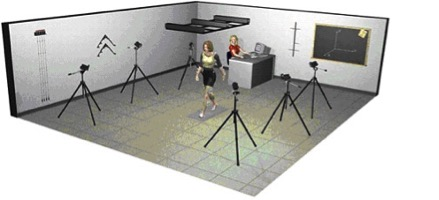
\includegraphics[width=0.9\textwidth]{./graphics/camera}
		\caption{Sistema de medida mediante cámaras} \label{fig:camera}
	\end{figure}
	
	\subsection{Sistemas optoelectrónicos}
	
	Los sistemas optoelectrónicos captan señales luminosas de marcadores colocados en el cuerpo del sujeto a medir y las convierten en señales eléctricas (ver Figura \ref{fig:opt}). A pesar de que se trata de un completo y minucioso método de análisis de la marcha, no resulta muy práctico en el ámbito del análisis clínico. Al alto coste y complejidad del equipo hay que añadir el amplio espacio de trabajo necesario para mantener una línea de visión libre de obstáculos entre el sujeto y los sistemas de medida. Además, la complejidad y lentitud provocan que resulte tedioso el tomar varias medidas \cite{begona,opt}.
		\begin{figure}[H]
			\centering
			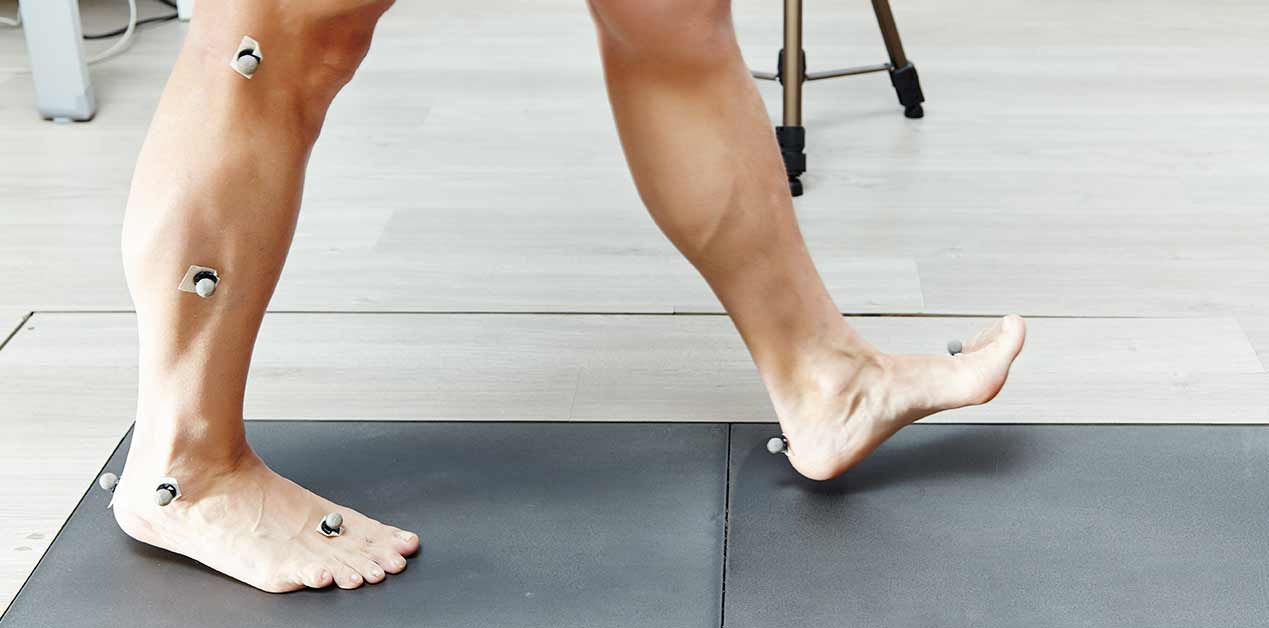
\includegraphics[width=0.9\textwidth]{./graphics/opt}
			\caption{Sistema de medida optoelectrónico} \label{fig:opt}
		\end{figure}

	\subsection{Tapices instrumentados}
	
	Existen sistemas como el GaitRite\textsuperscript{\textregistered} que permiten la medida de diferentes parámetros de la marcha, entre ellos la medida de distancia entre pasos \cite{gaitrite}. En la Figura \ref{fig:gaitrite} se observa dicho sistema el cual consiste en un tapiz instrumentado. Tiene como ventaja la portabilidad y la facilidad de manejo, así como el ahorro de tiempo debido a la automatización en el cálculo de los parámetros obtenidos. Sin embargo, existen ciertas limitaciones, dado que sólo se
	obtiene información de la presión ejercida sobre los sensores, sin tener en cuenta la
	dirección ni las componentes del vector de fuerza \cite{begona}. 
	
	\begin{figure}[H]
		\centering
		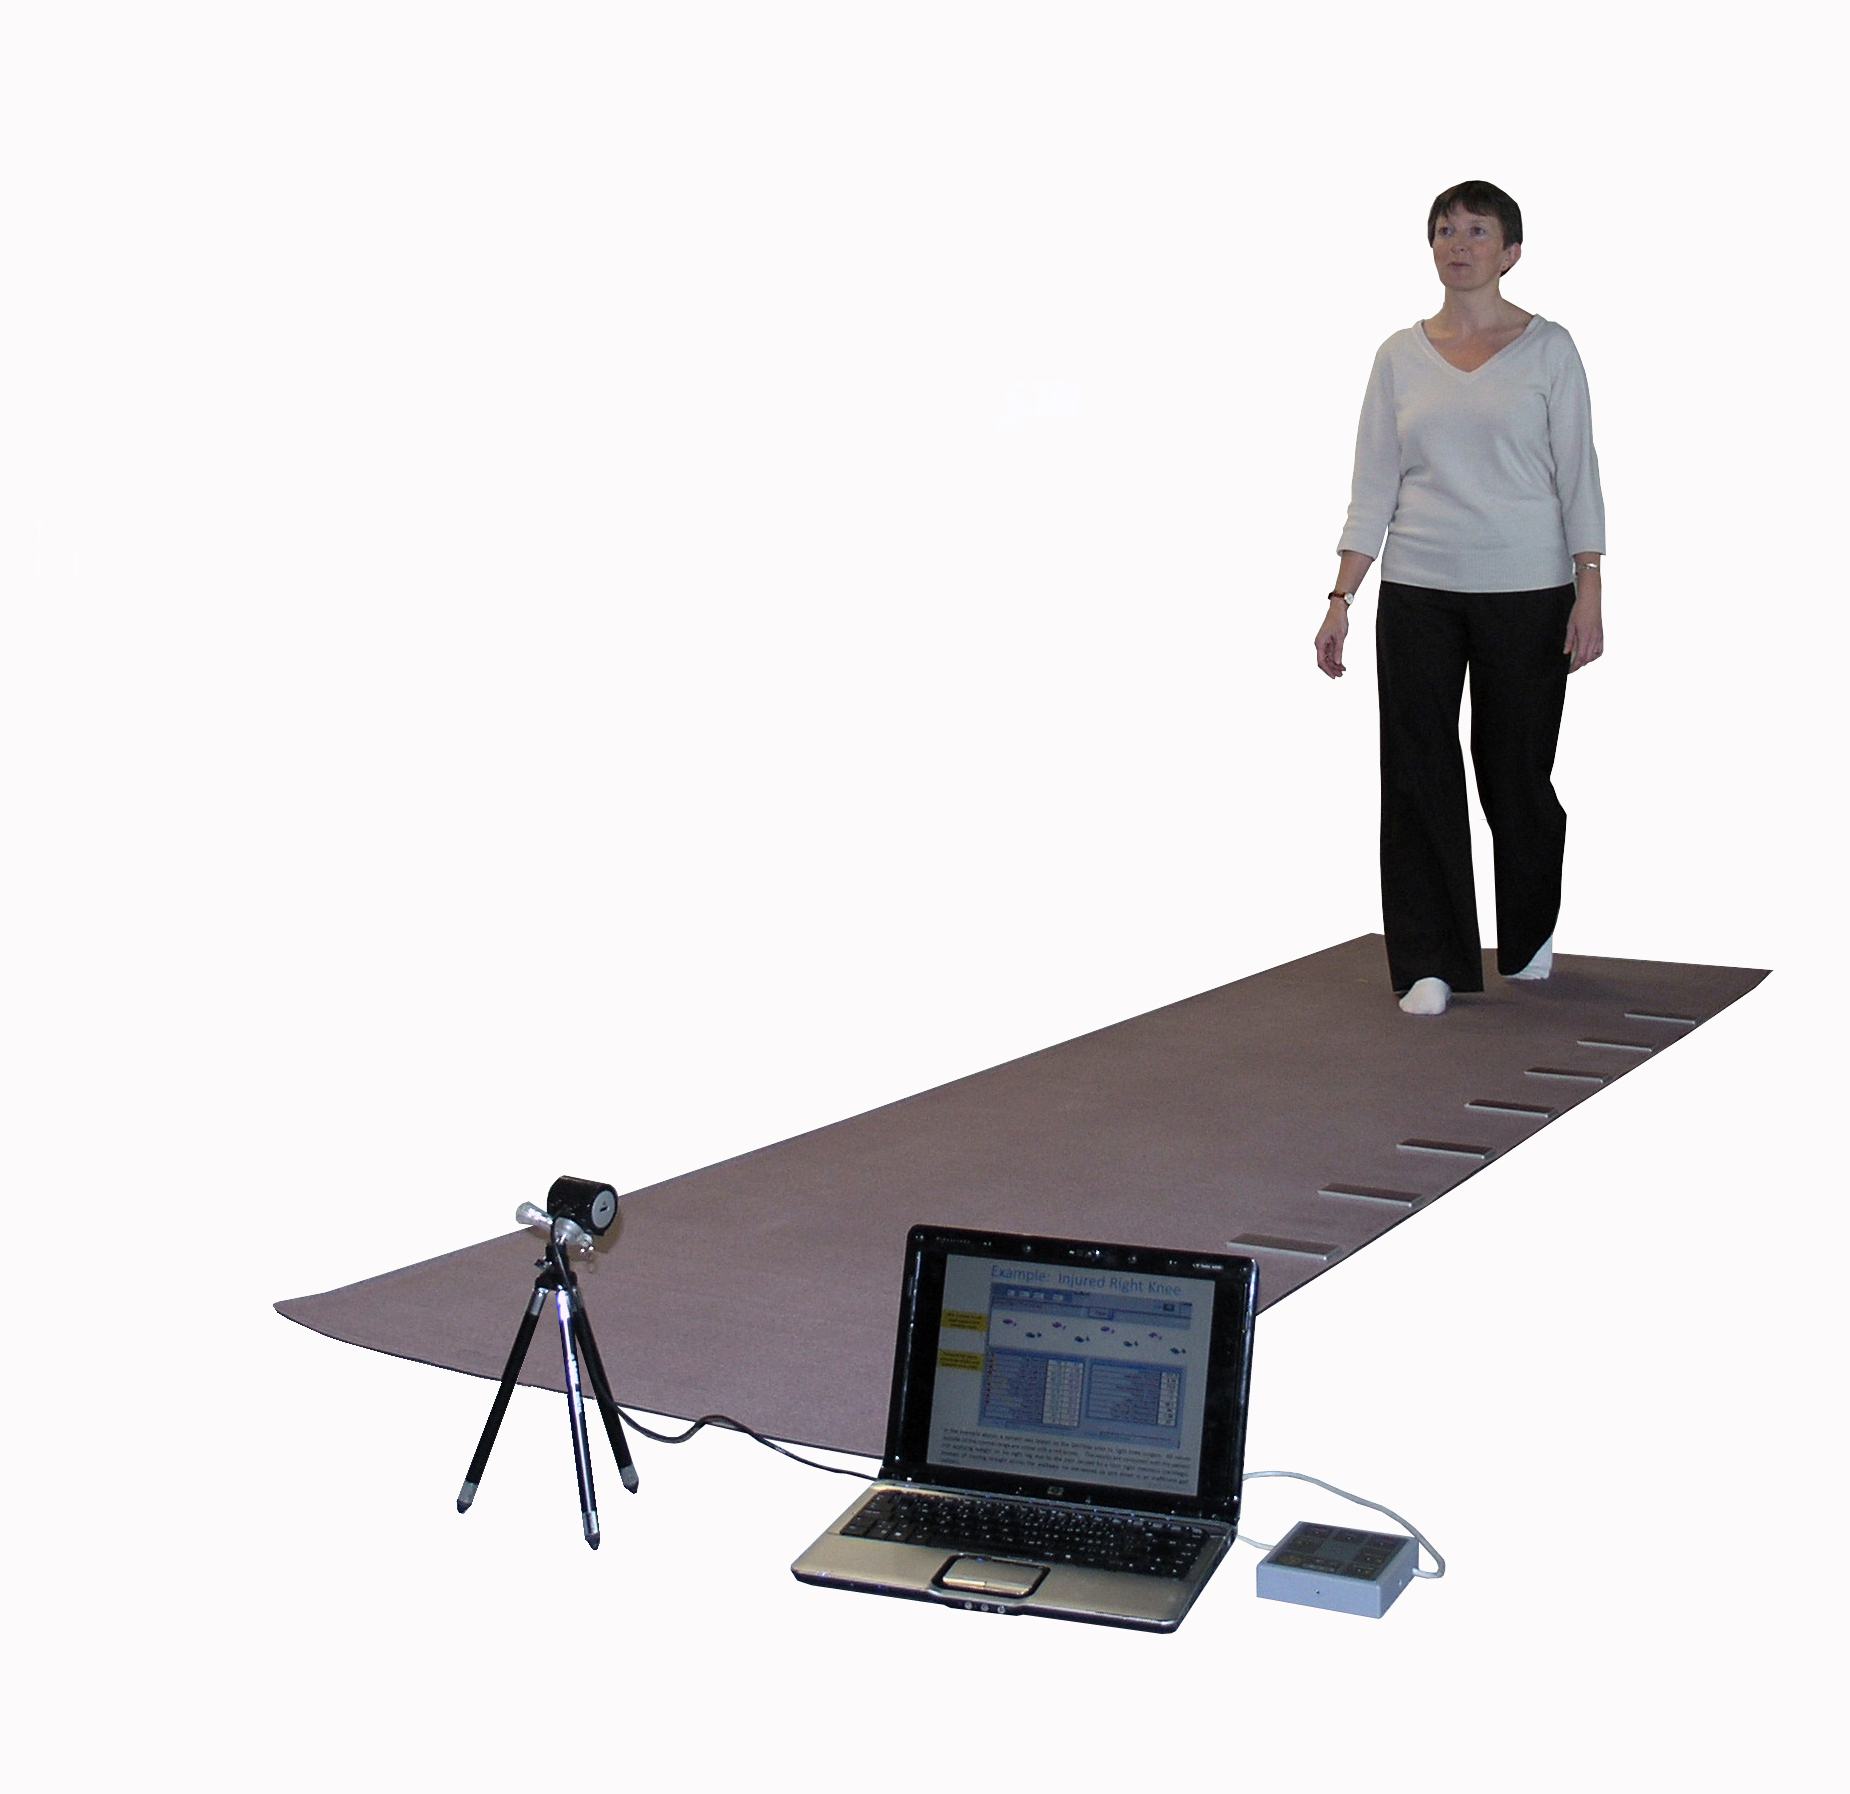
\includegraphics[width=0.6\textwidth]{./graphics/GaitRite}
		\caption{Sistema de medida GaitRite\textsuperscript{\textregistered}} \label{fig:gaitrite}
	\end{figure}
	
	\subsection{Zapatos instrumentados}
	
	\cite{shoes} Existe un sistema de medida integrado en zapatos que combina la utilización de sensores inerciales así como sensores de fuerza que completan la medida de los parámetros de la marcha. Se trata de un diseño compacto y que puede ser utilizado en entornos diferentes. En la Figura \ref{fig:shoes} aparece representado el diseño del zapato utilizado.
	
		\begin{figure}[H]
			\centering
			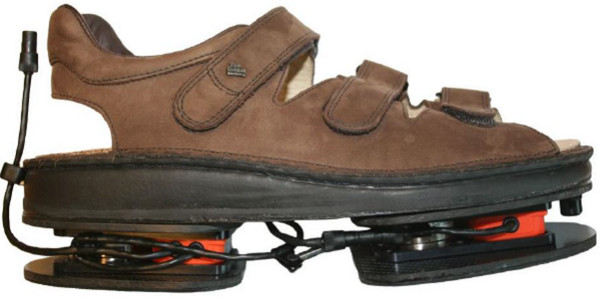
\includegraphics[width=0.6\textwidth]{./graphics/shoes}
			\caption{Zapatos instrumentados} \label{fig:shoes}
		\end{figure}
		 

Cada uno de los zapatos tienen un peso de aproximadamente 1.1Kg por lo que pueden afectar en la marcha a los pacientes ya que existe gran probabilidad de que hayan perdido fuerza en alguno de los lados. Además, únicamente con estos zapatos no es posible el cálculo de la distancia entre pasos por lo que aparecen nuevas versiones en las que se añaden sensores de ultrasonidos y por tanto reducen la ergonomía del sistema  \cite{shoes} . 


	
	
	
\thispagestyle{empty}
%
% Diseño
%
\chapter{Desarrollo del proyecto\label{sec:disenho}}

Para la realización de este trabajo se han tomado dos de las tecnologías expuestas en el capítulo \ref{sec:estado_del_arte} y se han llevado a la práctica. De esta manera se puede trabajar empíricamente con dos tecnologías diferentes planteadas como solución para un mismo problema. Una vez realizado todo el trabajo experimental se puede proceder a evaluar las características prácticas de cada tecnología y compararlas entre ellas. 

En función de la tecnología en que la se apoya cada uno de las soluciones, %por un lado se estudian los sensores de fibra FBG, capítulo \ref{sec:FBG3}, y por otro lado, los sensores IMU, capítulo \ref{sec:IMU3}.  
este capítulo se estructura de la siguiente manera: 
\begin{itemize}
	\item {\textbf{\ref{sec:FBG3}}    .- Solución con sensores de fibra FBG} 
	\item {\textbf{\ref{sec:IMU3}}    .- Solución con sensores IMU}
\end{itemize}




Dentro de cada punto se detalla toda la información necesaria para la implementación de cada uno de los sistemas. En ambos casos, la exposición de la solución tomada se divide en la explicación teórica en el \textit{Marco conceptual} y el ensayo práctico en el \textit{Desarrollo del prototipo}. El desarrollo del prototipo estudia los materiales empleados, el proceso de fabricación y el funcionamiento.  

%------------------------------
%------___SOLUCIÓN_FBG___------
%------------------------------
\section{Solución con sensores de fibra FBG}
\label{sec:FBG3}

\textcolor{rositaoscuro}{
	\textit{
		\colorbox{yellow}{Introducción} breve del guante, que tecnologias implica.
		Resumen fibras de Bragg 
		¿Qué es una fibra FBG?
		¿Porque se utilizan?
		El procesado de las señales resultantes se realiza mediante Labview.
	}
}


 Como primer prototipo se ha estudiado y llevado a cabo un guante cuyo funcionamiento se basa en los sensores de fibra FBG. 
 
 El prototipo consiste en una sección de PDMS con forma de huella de mano que tiene embebida una red en fibra de Bragg. Para la obtención, procesado y visualización de los resultados medidos se emplea el entorno de desarrollo LabVIEW.


%--Marco conceptual
\subsection{Marco conceptual}
\label{sec:mc3FBG}

Este apartado tiene por finalidad realizar una clara exposición de los conceptos teóricos fundamentales para la comprensión del diseño llevado a cabo. 

\begin{itemize}
%--FIBRA ÓPTICA
	\item \textbf{Fibra óptica}
	
	\textcolor{rositaoscuro}{
		\textit{
			Cómo se propaga la luz en ella.\\
	 		- -Partes de la fibra.\\
			Tipos de emisores (LED Laser).\\
			Receptores.\\
			Conectores.\\
			- -Fabricación.\\
			Soldado.\\
			- -Tipos de fibra.\\
		}
	}

	La fibra óptica es una hebra de material dieléctrico, así cómo el vidrio (sílice) o el polímero acrílico. 
	Se emplea como medio de propagación de señales luminosas. Es decir, para transmitir ondas electromagnéticas del espectro óptico: regiones espectrales de infrarrojo, luz visible y ultravioleta. En la siguiente imagen (figura \ref{fig:espectroOptico}) se puede observar dentro del espectro electromagnético dónde se sitúa el espectro óptico.	 
	\begin{figure}[H]
		\centering
		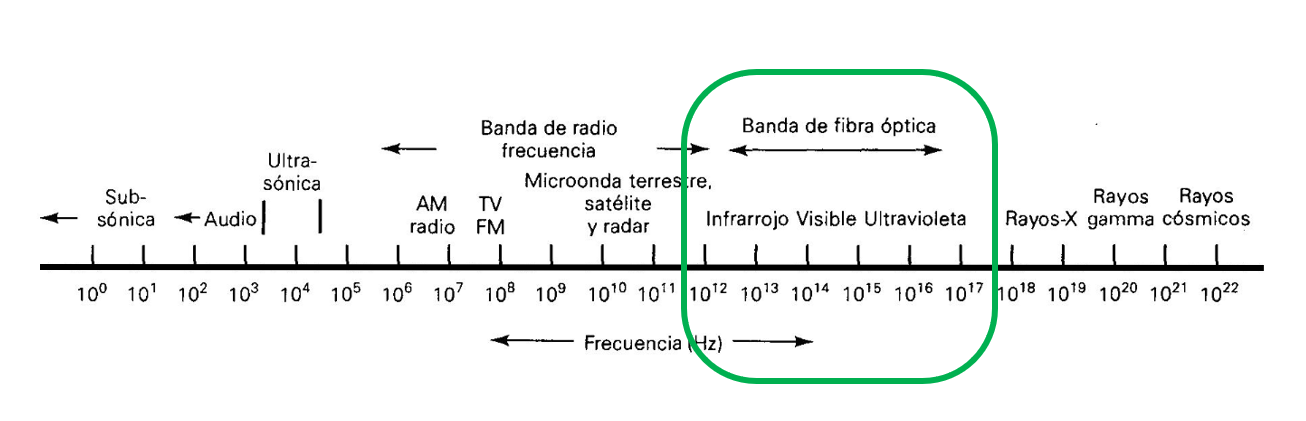
\includegraphics[width=0.95\textwidth]{./img/espectrooptico}
		\caption{Espectro electromagnético en frecuencia.}
		\label{fig:espectroOptico}
	\end{figure}

	Cabe destacar que dentro del espectro óptico las longitudes de onda habituales para comunicación en fibra óptica están entre los 700nm y 1600nm. Estas se dividen en rangos con mejores características para la transmisión, denominadas ventanas de comunicación. Como se muestra en la figura \ref{fig:ventanaOptica}, son tres las ventanas más utilizadas,\cite{ventanasFO}:
%	\begin{itemize}
%		\item \textbf{1ª ventana}\hspace{0.2cm} 800 a  900 nm tilizada  =  850nm
%		\item \textbf{2ª ventana}\hspace{0.1cm}  1250 a 1350 nm   l utilizada  = 1310nm
%		\item \textbf{3ª ventana}\hspace{0.1cm}  1500 a 1600 nm   l utilizada  = 1550nm 
%	\end{itemize}
	
	\begin{table}[H]
		%\centering
		\hspace{2cm}
		\renewcommand{\arraystretch}{2}
		\begin{tabular}{rrl}
			\textbf{1ª ventana}& 800 a  900 nm  & $\longmapsto$ $\,$ longitud de onda utilizada = 850nm  \\
			\textbf{2ª ventana}& 1250 a 1350 nm & $\longmapsto$ $\,$ longitud de onda utilizada = 1310nm  \\
			\textbf{3ª ventana}& 1500 a 1600 nm & $\longmapsto$ $\,$ longitud de onda utilizada = 1550nm   \\ 
		\end{tabular} 
	\end{table}

	 \begin{figure}[H]
	 	\centering
	 	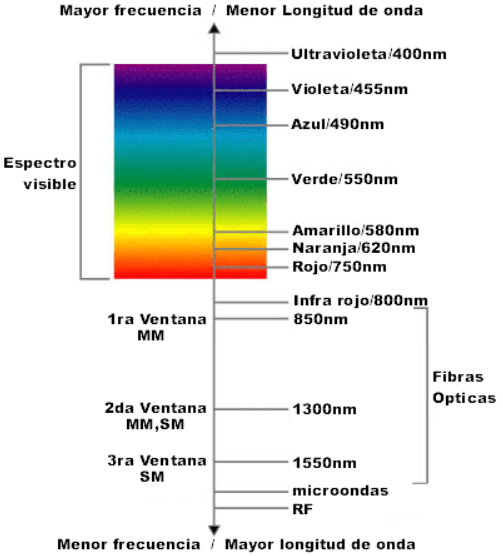
\includegraphics[width=0.5\textwidth]{./img/ventana}
	 	\caption{Longitud de onda fibra óptica junto con el espectro visible. \cite{ventanasFO}}
	 	\label{fig:ventanaOptica}
	 \end{figure}
 
 En cuanto a las propiedades físicas de la fibra óptica, son bastante delicadas ya que su grosor no supera por mucho al diámetro del cabello humano y se obtiene de la extrusión del sílice, SiO\textsubscript{2} , es decir, se trata de un filamento de vidrio muy fino. Es por ello que es la fibra óptica estándar está rodeada de una cubierta protectora. 
 
  \begin{figure}[H]
  	\centering
  	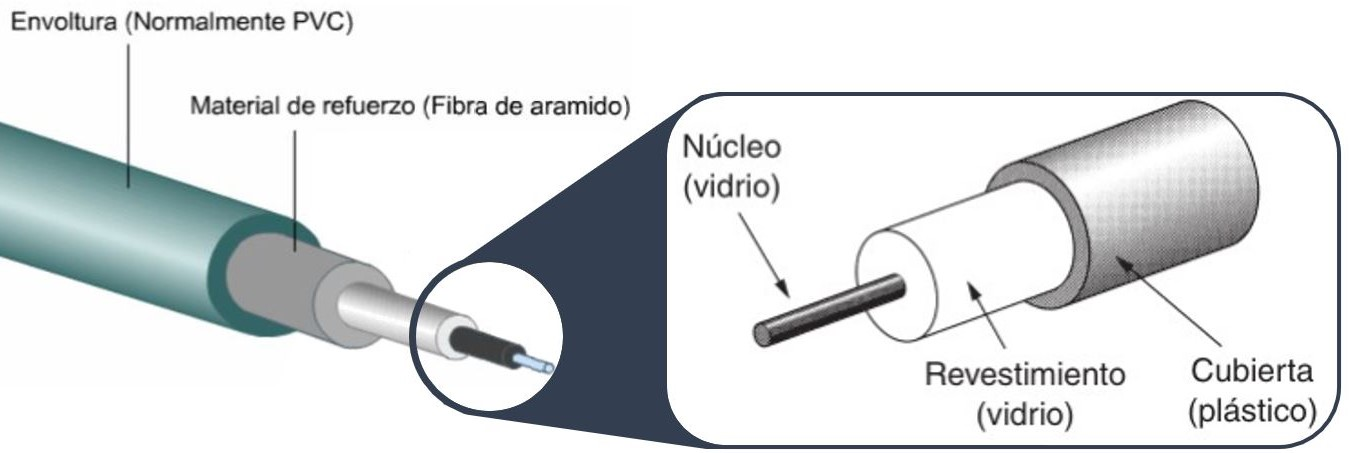
\includegraphics[width=0.87\textwidth]{./img/capas-fibra2}
  	\caption{Capas fibra óptica \cite{imgNucleoFibra,imgCapasFO}} 
  	\label{fig:capasFibra}
  \end{figure} 
  
  
  
 La fibra óptica estándar cuenta varias capas (figura \ref{fig:capasFibra}): núcleo, revestimiento y cubierta (o buffer).  Si la aplicación lo permite, conviene proteger la fibra con más capas externas. En la imagen anterior la fibra está además protegida por un material de refuerzo (fibra de aramido) y una envoltura (PVC).
 
 Tanto el núcleo cómo el revestimiento forman el medio por el cual se propaga la luz. Estas dos capas son tan finas que forman un filamento flexible, pero muy delicado, puesto que es muy propenso a romperse ante dobleces u otras manipulaciones externas. Por ello el resto de las capas son tambien importantes por proporcionar a la fibra protección y haciendo posible su utilización es escenarios de despliegue.
 
 La fabricación de la fibra óptica es un proceso de alta tecnología. Es importante mantener la pureza y la regularidad del núcleo. Esto es complejo, puesto que estamos hablando en algunos casos de núcleos de un grosor entorno a las 8 micras (en fibras monomodo). El grosor estándar de la fibra es de 125 micras(una micra equivale a una millonésima parte de un metro). Para conseguir este resultado el proceso de fabricación consiste en reproducir a escala macroscópica la estructura de la fibra que se quiere obtener. Esta reproducción a gran escala de la fibra deseada se le denomina preforma. Una vez se tiene la preforma, esta se va fundiendo y estirando hasta alcanzar el filamento del diámetro deseado. De una preforma se pueden sacar kilómetros de fibra. Para fabricar la preforma se parte de una barra de vidrio hueca (el vidrio que formará el recubrimiento) y se baña en un gas que contiene unas partículas (lo que formará el núcleo). Al calentar a mil grados, las partículas comienzan a fundirse hasta que el tubo colapsa y forma una vara maciza, que es la preforma. Para fundirla y estirarla esta se coloca verticalmente y se calienta. La complejidad de esta fase reside en mantener constante el flujo y el diámetro del hilo resultante. Además durante esta fase se aprovecha para crear una capa protectora sobre el vidrio (cubierta en la figura \ref{fig:capasFibra}). Finalmente los kilómetros de fibra óptica se enrollan en grandes bobinas. \cite{fabricacionFO}
 
  \begin{figure}[H]
 	\centering
 	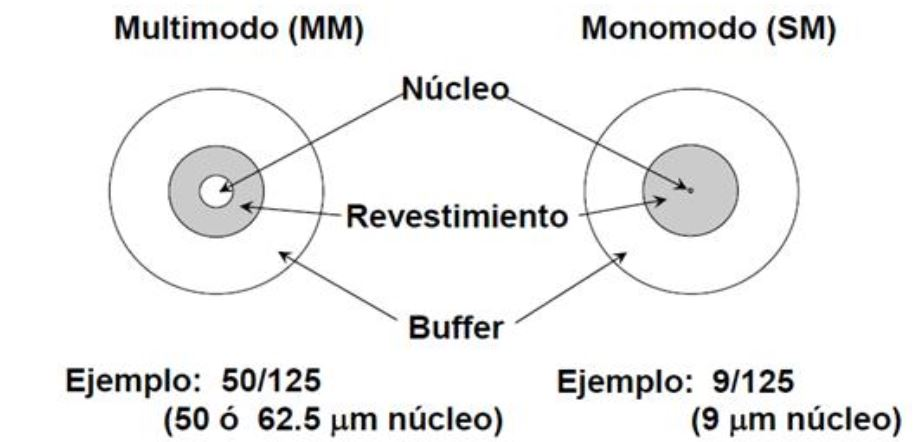
\includegraphics[width=0.6\textwidth]{./img/MM-SM}
 	\caption{Relación grosor fibra multimodo (MM) y monomodo (SM) \cite{imgRadioModo} } 
 	\label{fig:modoMonoMulti}
 \end{figure} 
 
  Dependiendo de la relación de diámetro entre el núcleo y el revestimiento, la fibra fibra será monomodo o multimodo (figura \ref{fig:modoMonoMulti}). Esta diferencia afecta a la propagación de la luz dentro de la guía de onda. Ya se ha comentado que el diámetro de la fibra es de aproximadamente 125 micras. En el caso de las fibras monomodo, el núcleo de estas tiene un diámetro tan pequeño (en torno a 8 micras) que la luz solo puede propagarse en un sólo modo (rayo). Sin embargo, en el caso de las fibras multimodo, al poseer un núcleo mayor (entre 50 o 62.5 micras) soportan la transmisión el múltiples modos, es decir, los rayos de luz viajan en muchas direcciones a través de este. \cite{FOA} 
   
  	\textcolor{rositaoscuro}{revisar:}
 	\begin{figure}[H]
		\centering
		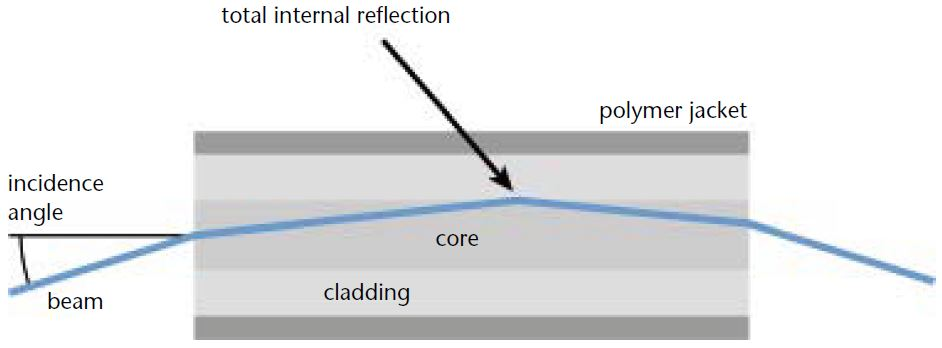
\includegraphics[width=0.5\textwidth]{./img/guiaMM}
		\caption{Guía de un haz de luz en una fibra multimodo a través de la reflexión interna total en la interfaz núcleo-revestimiento. \cite{imgMonoMulti} } 
		\label{fig:guiaMM}
	\end{figure} 
  	\begin{figure}[H]
		\centering
		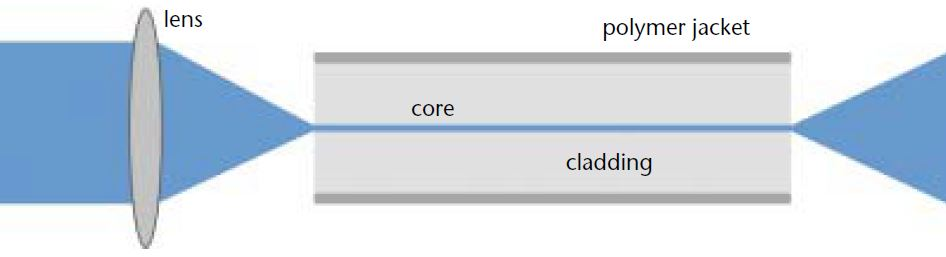
\includegraphics[width=0.7\textwidth]{./img/guiaSM}
		\caption{Orientación de la luz en una fibra monomodo. El perfil de intensidad dentro del núcleo está determinado únicamente por el diseño de la fibra. \cite{imgMonoMulti} } 
		\label{fig:guiaSM}
	\end{figure}  
 	
 	\textcolor{rositaoscuro}{\textit{Si veo que tal puedo extenderme con relacionar las \underline{ventanas con monomodo y multimodo}. Y además concretar mas las \underline{características de cada ventana} (gráfica de interferencias esta)}\\
 	\\Generalmente, la fibra multimodo se utiliza con fuentes LED en longitudes de onda de 850 y 1300 nm (ver debajo) para redes de área local (LAN) más lentas y con fuentes láser a 850 nm (VCSEL) y 1310 nm (láser Fabry-Perroy) para redes que operan a velocidades de gigabits por segundo o mayores. \\
	La fibra monomodo se utiliza para telefonía y para televisión por cable (CATV) con fuentes de luz láser a 1300 y 1550 nm ya que tiene poca pérdida y un ancho de banda prácticamente infinito.\\
	Existen otros tipos de fibras opticas: POF - PCS y HCS (imagen ejemplo de diámetros).}

 La diferencia de índices de refracción entre las capas centrales de la fibra son las que permiten la propagación de la luz a través de esta. El índice de refracción del núcleo es mayor que el del revestimiento.
 
\cite{geometriaBasicaFP}
 
 
 
  \textcolor{rositaoscuro}{//explicar más REFRACCIÓN}

  Puesto que en la solución con estudiada en este trabajo se utilizan fibras monomodo no se va a extender el texto en explicar más conceptos sobre la transmisión en fibras multimodo.
 
 
 Los sistemas de propagación de señales luminosas a través de la fibra óptica componen un medio de transmisión de datos rápido y fiable. Previa a la propagación a través de un medio óptico de una señal eléctrica (analógica o digital) es necesario realizar una conversión de esta a señal óptica. Esto genera una señal óptica a partir de una señal eléctrica en el emisor o fuente de luz situado en el extremo inicial de la comunicación. Realizada la conversión, la señal es transmitida a lo largo de la fibra óptica. Según las características del escenario puede haber una o varias uniones entre fibras a lo largo del canal. Estás pueden realizarse empalmando o utilizando conectores. Una vez la señal óptica atraviesa todo el canal, llega al detector, dónde sucede el proceso inverso al ocurrido en el emisor y a la salida del sistema completo se tiene la señal eléctrica. Esta corresponde a la señal introducida al sistema con una pequeña posibilidad de haber sufrido pérdidas o atenuación debido a la impureza de la fibra, la distancia, las conexiones entre elementos del sistema o cualquier otro evento ajeno al este. Estas modificaciones de la señal de entrada pueden ser contrarrestadas o solventadas en recepción sin suponer un impedimento a una comunicación exitosa. (figura \ref{fig:TxFOp2p})
 
   \begin{figure}[H]
 	\centering
 	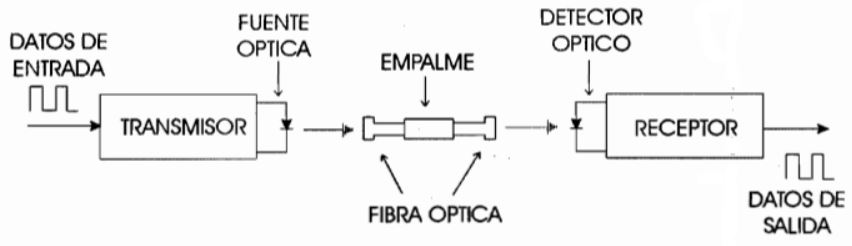
\includegraphics[width=0.75\textwidth]{./img/TxFOp2p}
 	\caption{Transmisión punto a punto de señales a través de fibra óptica. \cite{txFO} } 
 	\label{fig:TxFOp2p}
 	\end{figure} 

 Veamos por separado los elementos dibujados en la figura \ref{fig:TxFOp2p}:
 	\begin{itemize}
 		\item \textit{\textbf{Emisores (Transmisión)}}	
 		% \hspace{0.2cm} 
 		
 		\item \textit{\textbf{Detectores (Recepción)}}
 			
 			
 		\item \textit{\textbf{Conectores y empalmes}}
 		
 	 \end{itemize}
 


					//--\\						
					La propagación de la luz desde el punto inicial hasta el extremo final se debe al fenómeno de
					reflexión total interna [20] de la luz. Este hecho tiene lugar cuando un haz de luz trata de
					pasar de un medio de mayor índice de refracción, n1, a uno de menor índice de refracción, n2,
					y con un ángulo determinado (Fig. 3.3.). El ángulo de incidencia debe superar el valor crítico.
					Cuando se dan estas condiciones, el rayo de luz incidente se refleja completamente, no
					pudiendo atravesar la frontera que separa ambos medios y volviendo nuevamente hacia el
					medio origen, con un ángulo de reflexión igual al ángulo de incidencia.
					
					
					En una fibra óptica, para provocar el fenómeno de reflexión total interna, se asegura que la luz
					penetra con una determinada apertura numérica, que es el ángulo necesario para forzar a la
					mayoría de los rayos de luz a incidir sobre la superficie de separación entre el núcleo y la
					cubierta. En estas condiciones, y de acuerdo con las leyes de Snell, los rayos de luz incidentes
					a esta interfaz de separación superan el ángulo crítico, pudiendo así reflejarse prácticamente
					en su totalidad a lo largo de toda la estructura.
					


---

TIPOS DE EMISORES


					///---
					LASER
					
					Para poder transmitir en una de estas ventanas es necesaria una fuente de luz "coherente", es decir de una única frecuencia (o longitud de onda), la cual se consigue con un componente electrónico denominado LD ó diodo LASER (Light Amplification by Estimulated Emision of Radiation). Este componente es afectado por las variaciones de temperatura por lo que deben tener un circuito de realimentación para su control.
					
					También pueden usarse diodos LED.
					
					Detectores ópticos
					
					Como receptores ópticos se utilizan fotodiodos APD o diodos pin (PIN-PD) que posen alta sensibilidad y bajo tiempo de respuesta.
					
					El APD también requiere de un ajuste automático ante variaciones de temperatura.


\textcolor{teal}{
	Recubrimientos: http://apacoe.weebly.com/conocimiento/que-es-la-fibra-optica
	Link:Conectores y empalmes
	http://www.thefoa.org/ESP/Conectores.htm
}

%-- REDES DE DIFRACCIÓN DE BRAGG	
	\item \textbf{Redes de difracción de Bragg}
		
	Funcionamiento y sensibilidad
	
%-- POLIDIMETILSILOXANO - PDMS	
	\item \textbf{Polidimetilsiloxano (PDMS)}
		
	Material empleado para embeber las FBGs.
	
%-- LABVIEW 	
	\item \textbf{LabVIEW}
		
	LabVIEW es un software de ingeniería de sistemas que requiere pruebas, medidas y control con acceso rápido a hardware e información de datos. \cite{LabVIEWpage}





\end{itemize}
 
%--Desarrollo del prototipo
\subsection{Desarrollo del prototipo}
\label{sec:prot3FBG}
%[Esta parte de desarrollo del proyecto parte de otro trabajo. Aquí mencionar algo que diga el trabajo de Silvia y mencionar la en la bibliografía.]

La realización del primer desarrollo se origina a partir de un trabajo realizado con anterioridad en el grupo de investigación de la universidad\cite{SilviaTFM}. Se mejora el soporte físico(hardware) y se desarrolla un nuevo programa con un interfaz de usuario simple e intuitivo.

El prototipo consiste en un prototipo técnico y funcional de un guante, con sensores de FBG embebidos en PDMS. 
 
\subsubsection{Materiales}
En este apartado se disponen brevemente los componentes utilizados para el 
\begin{figure}[H]
	\centering
	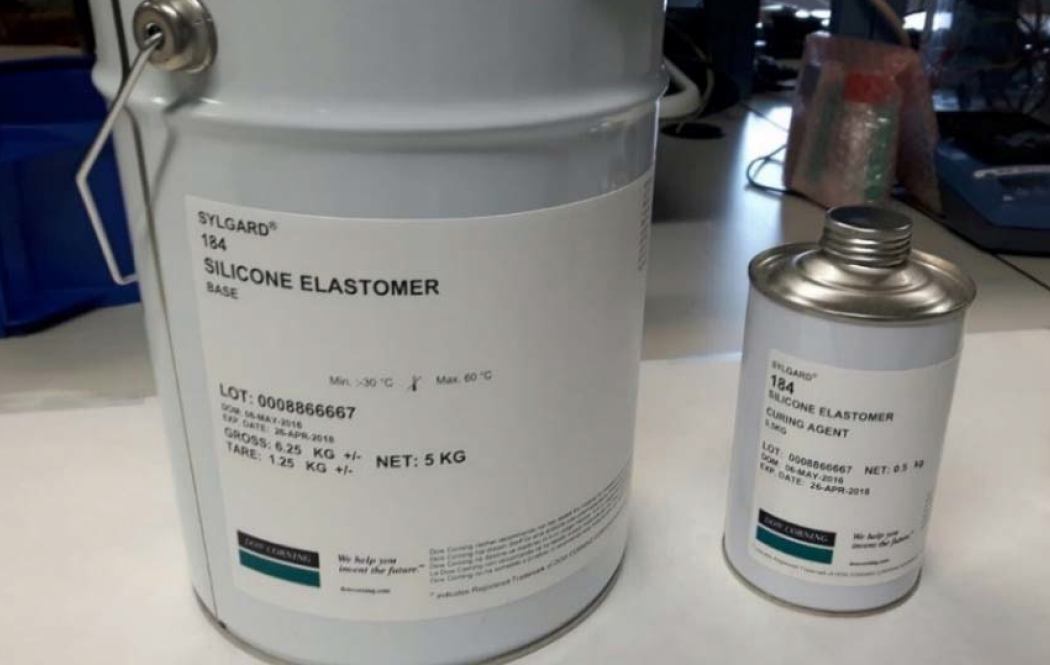
\includegraphics[width=0.75\textwidth]{./img/PDMS}
	\caption{PDMS: Elastómero y agente de cura.} \label{fig:pdms}
\end{figure}



\subsubsection{Proceso de fabricación del soporte físico}
%Elaboración
Para que sea más cómoda la explicación del proceso de elaboración del prototipo se divide este en tres partes: modelado 3D, fabricación del guante y montaje de prototipo completo.

\begin{itemize}
	\item \textbf{Modelado 3D - Configuración 3D}
	
	Esta actividad comprende el diseño del molde con el que se fabrica el guante y de la caja contenedora de todo el cableado.
	Para poder producir el guante de PDMS es necesario tener un molde donde verter la disolución para darle la forma deseada. Gracias a las versatilidad de diseño que ofrece la impresión 3D se realiza con este proceso de manufactura el molde (véase figura \ref{fig:molde}). 
\begin{figure}[H]
	\centering
	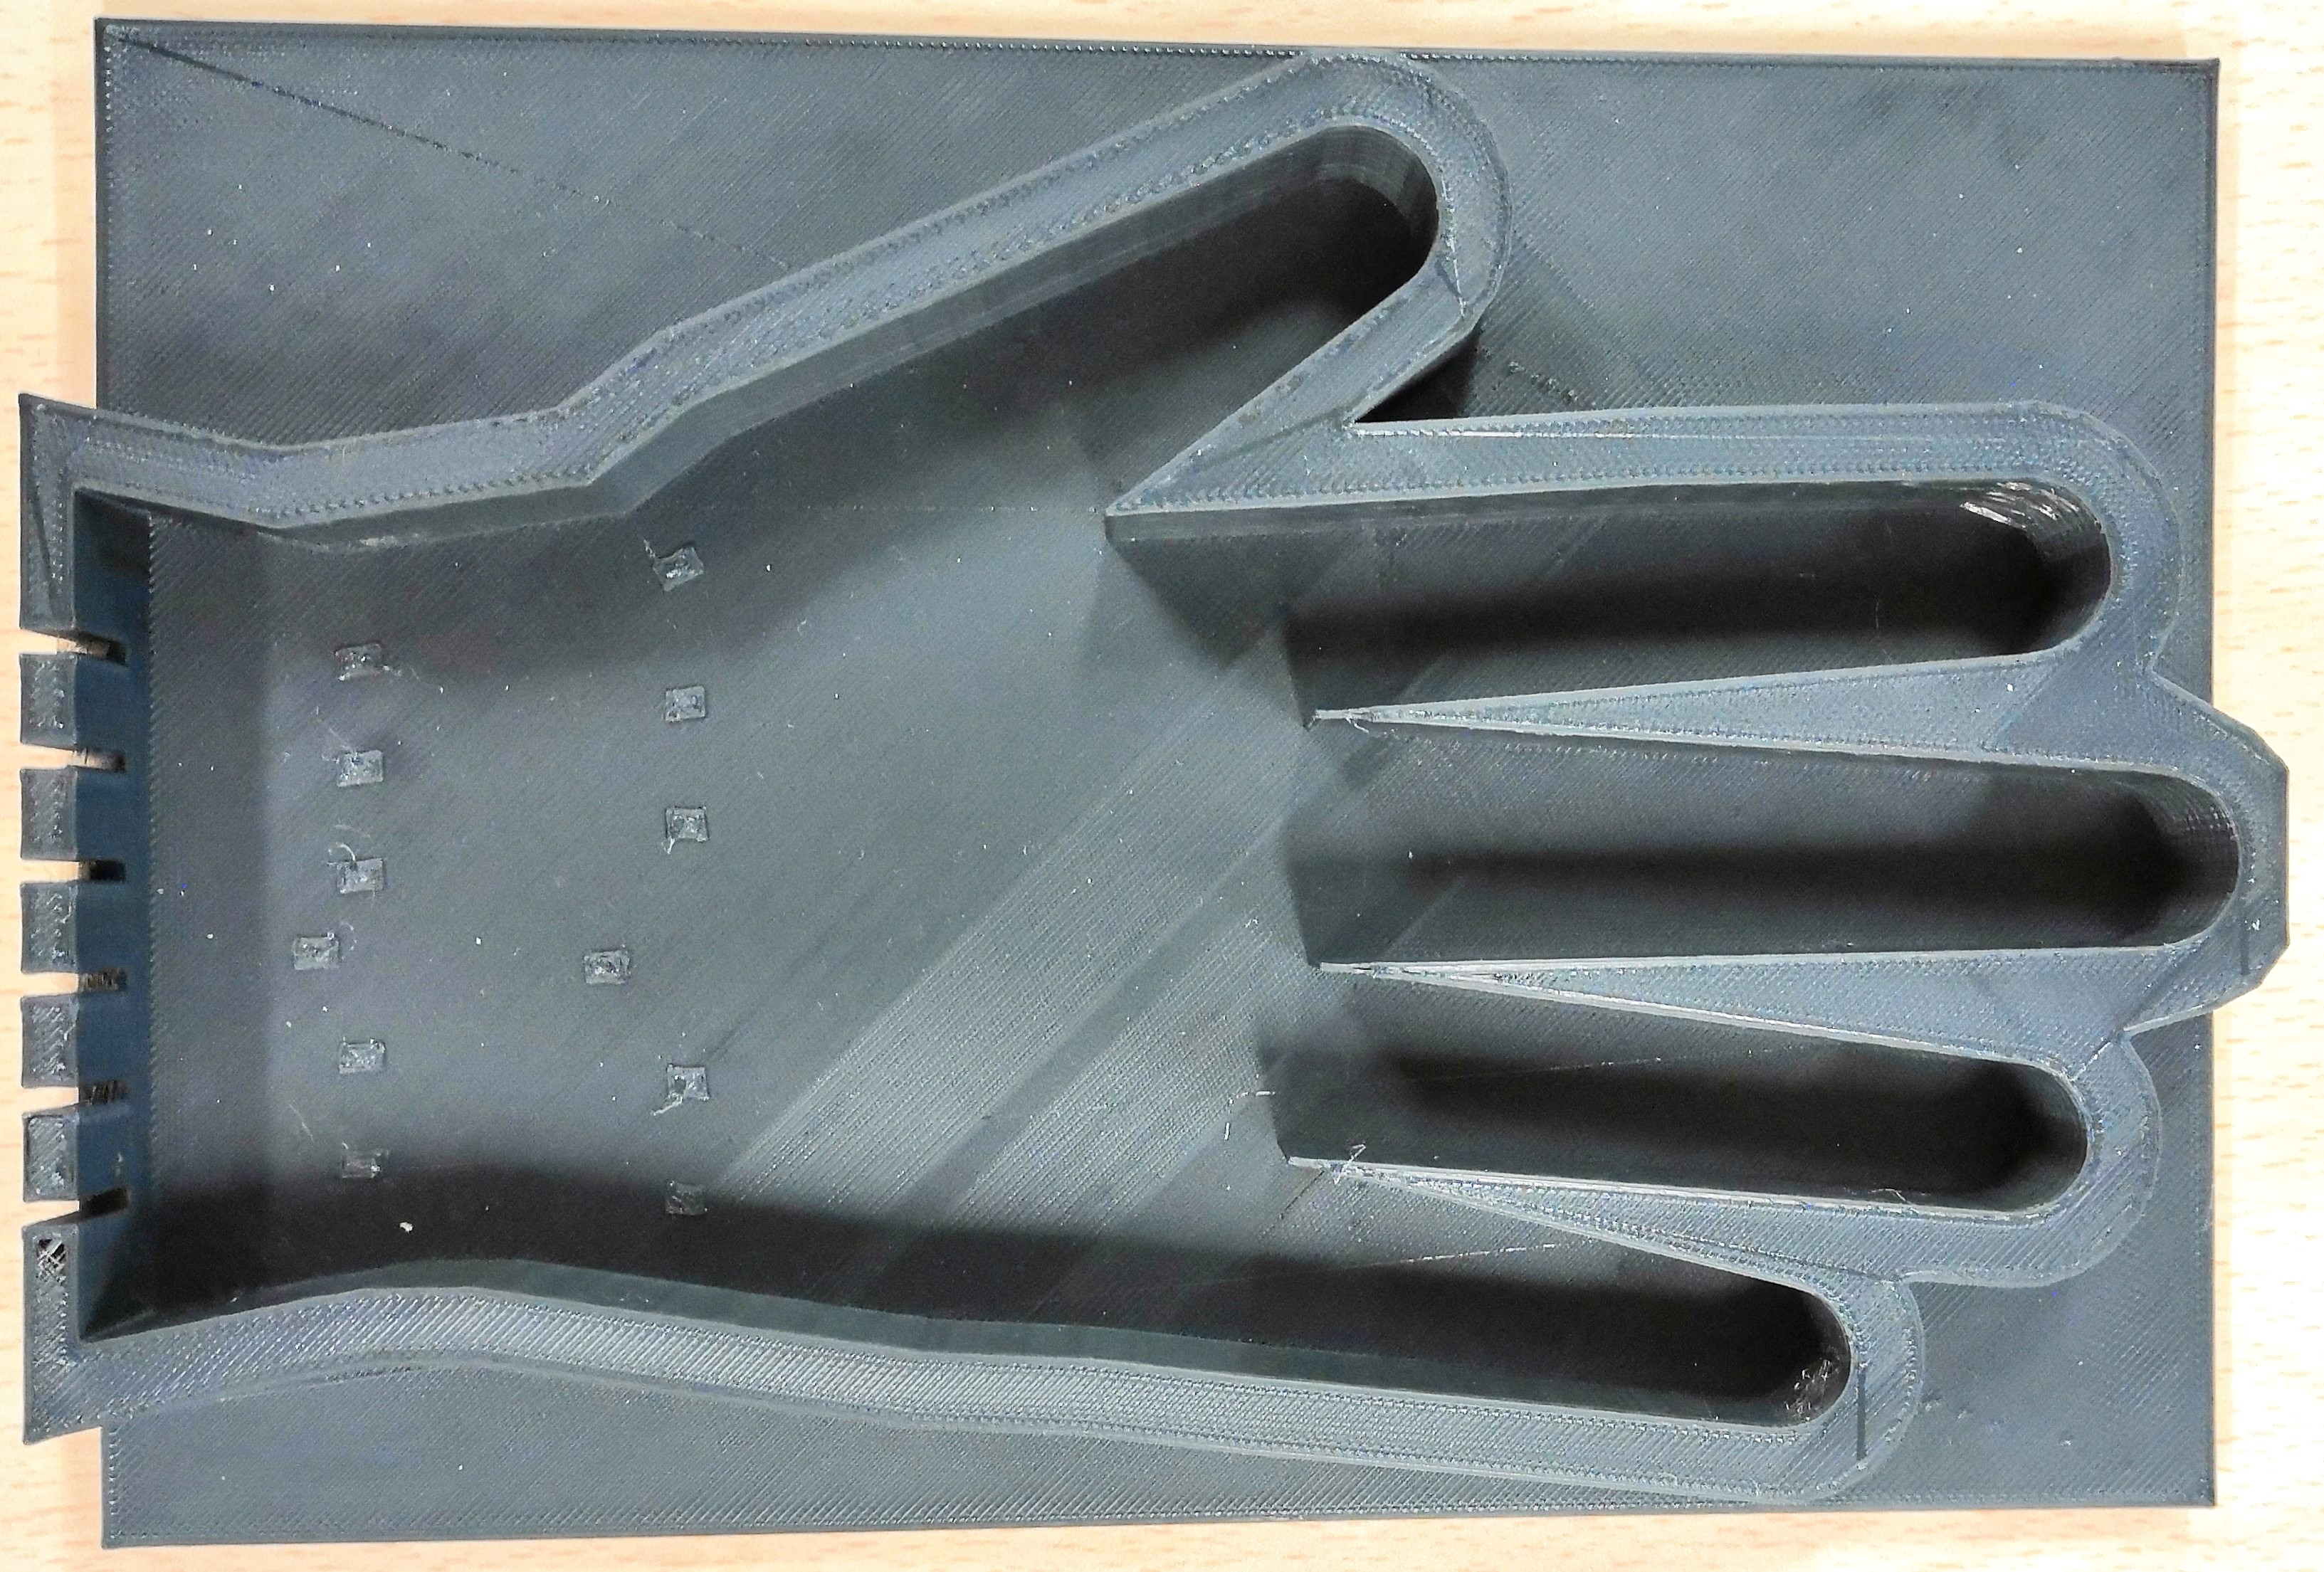
\includegraphics[width=0.5\textwidth]{./img/molde1}
	\caption{Molde} \label{fig:molde}
\end{figure}

	
 
	\item \textbf{Fabricación del guante}
	
	Para el proceso de fabricación del guante se necesitan ..................
	
	\begin{enumerate}
		\item Preparar mezcla PDMS (35g de polímero y 3.5g de agente de curación). Primero el
		elastómeto y después agente de curación.
		\item Revolver la mezcla durante al menos 4 minutos.
		\item Se deposita el PDMS y se colocan las fibras en el molde
		\item Se introduce en un horno de vacío para eliminar las burbujas durante 20 minutos, sin aplicar
		temperatura.
		\item Meter el molde en el horno (4h y media a $-55\,^{\circ}\mathrm{C}$). Dejar un poco más.
		\item Desmoldar.

	\end{enumerate}
	
	
	\item \textbf{Montaje completo}
	
	asdf
	
\end{itemize}

asdf





\begin{table}[H] %BORRAR
	\centering
	\begin{tabular}[t]{|c|}
		\hline
		\textbf{\textcolor{rositaoscuro}{BORRAR}} \\
		\hline
		longitudes de onda del guante de fibras cortas\\
		\hline
	\end{tabular}
	\begin{tabular}[t]{|r|c|}
		\hline
		 & Longitud de onda del sensor\\
		\hline
		\hline
		Dedo pulgar & 1512 nm \\
		\hline
		Dedo índice & 1520 nm \\
		\hline
		Dedo corazón & 1528 nm \\
		\hline
		Dedo anular & 1536 nm \\
		\hline
		Dedo meñique & 1544 nm \\
		\hline
		Muñeca & 1556 nm \\
		\hline
	\end{tabular}
	\caption{Tabla longitud de cada sensor FBG}
	\label{tabla:medidas 80 cm}
\end{table}
%-- Hasta aquí borrar la tabla.


\begin{table}[H]
	\centering
	\begin{tabular}[t]{|r|c|}
		\hline
		& Longitud de onda del sensor\\
		\hline
		\hline
		Dedo pulgar & 1532 nm \\
		\hline
		Dedo índice & 1548 nm \\
		\hline
		Dedo corazón & 1576 nm \\
		\hline
		Dedo anular & 1568 nm \\
		\hline
		Dedo meñique & 1560 nm \\
		\hline
		Muñeca & 1541.26 nm \\
		\hline
	\end{tabular}
	\caption{Tabla longitud de cada sensor FBG}
	\label{tabla:medidas 80 cm}
\end{table}

Para determinar la valid


\subsubsection{Funcionamiento}
asdf

\begin{figure}[H]
	\centering
	\includegraphics[width=1\textwidth]{./img/interfazSM}
	\caption{Interfaz del programa de labview.}
	\label{fig:interfaz}
\end{figure}

%------IIIIIIMMMMMMUUUUUU------
\section{Solución con sensores IMU}
\label{sec:IMU3}
asdf

\subsection{Marco conceptual}
\label{sec:mc3IMU}
asdf

\subsection{Desarrollo del prototipo}
\label{sec:prot3IMU}
asdf

\subsubsection{Materiales}
asdf


\subsubsection{Elaboración/Proceso de fabricación}
asdf

\subsubsection{Funcionamiento}
asdf




\section{---------------}

ME PLENTEO LA POSIBILIDAD DE DIVIDIR EL CAPITULO 3 EN CAPITULO 3 Y 4.


----------------------------------------------------------------------------------------------------------------------------------------------------------------------------------------------------------------------------------------------------------------------------------------------------------------------------------------------------------------------------------------------------------------------------------------------------------------------------------------------------------------------------------------------------------------------------------------------------------------------------------------------------------------------------------------------------------------------------------------------------------------------------------------------------------------------------------------------------------------------------------------------------------------------------------------------------------------------------------------------------------------------------------------------------------------------------------------------------------------------------------------------------------------------------------------------------------------------------------------------------------------------------------------------------------------------------------------------------------------------------------------------


\section{---------------}















En este capítulo se detalla la metodología empleada para el diseño del sistema adaptado al contexto en el que se aplica. Se describe cada uno de los componentes que forman parte del sistema de medición así como el procesado posterior de los datos para obtener la distancia entre pasos(Matlab\textsuperscript{\textregistered}). En el diseño intervienen sensores inerciales (Xsens Technologies B.V, The Netherlands) y se propone el diseño de un sensor de ultrasonido de bajo coste basado en la tecnología Arduino. 


\section{Sistema de medida}
En la Figura \ref{fig:esquema} aparece representado un esquema general de la metodología empleada. Mediante el sensor de ultrasonidos se obtiene la distancia D1 y con los sensores inerciales se obtiene la distancia D2 aplicando a cada una de las señales el procesado que se detallará en posteriores apartados.


Por tanto, el diseño del sistema puede descomponerse en dos niveles de jerarquía  (ver Figura \ref{fig:esquemaniveles}). El primero de ellos, a más bajo nivel, es el diseño del sensor de ultrasonidos y la obtención de las señales necesarias para el cálculo de cada una de las distancias de ambos sensores. El segundo de los niveles es el correspondiente al de la sincronizcación y post-procesado de los datos para determinar la distancia entre pasos.

 Con el  post-procesado de las señales obtenidas por cada uno de los sensores se obtendrán las distancias D1 y D2 que permitirán el cálculo de la distancia objetivo mediante la ecuación \ref{eq:distancia} (Teorema de Pitágoras).

\begin{equation}\label{eq:distancia}
Dist.sep.pasos = \sqrt{D1^2 + D2^2}
\end{equation}


En los siguientes apartados se especifican cada uno de los componentes que intervienen en el sistema. 
\section{Sensores inerciales}
\subsection{Principio de funcionamiento}

Un sistema de referencia inercial se trata de un sistema de referencia regido por las leyes de movimiento de Newton. Por tanto, un sensor capaz de medir valores respecto a dicho sistema de referencia es lo que se conoce como un sensor inercial.

Una unidad inercial o IMU (Inertial Magnetic Unit) es un dispositivo que se compone de tres giróscopos (para determinar la orientación), tres acelerómetros y un reloj que permite asignar tiempo a los valores medidos por los sensores inerciales. Dichas unidades inerciales presentan tres ejes y cada uno de ellos presenta un acelerómetro y un giróscopo.

Por tanto, la información que se recoge de las unidades inerciales son aceleraciones lineales, velocidades angulares y tiempo común para los tres ejes que llevan dicha información de aceleración y velocidad angular (ver Figura \ref{fig:Imu}). 


El tiempo requerido para la implementación del sistema de medida puede influir en la marcha de los pacientes y por tanto en la obtención de los parámetros \cite{begona}. Los sensores inerciales utilizados permiten realizar las mediciones de una manera sencilla y rápida lo cual resulta beneficioso en el contexto ambulatorio tanto para los pacientes como para el personal sanitario



\subsection{Sensores inerciales propuestos}
Los sensores inerciales utilizados para el sistema son el modelo MTw Awinda (Xsens Technologies B.V, The Netherlands) pueden verse representados en la Figura \ref{fig:sensor_XSENS}



Su tamaño es de 47 x 30 x 13mm y 16g de peso por lo que puede definirse como un sistema compacto y ergonómico que será de utilidad para el sistema propuesto en este trabajo. Dispone de unas bandas de sujeción que permiten colocar el sensor en el lugar necesario y por tanto dota de versatilidad al diseño. 

Además, se incluye un software de captura que resultará útil para obtener las señales para su posterior procesado. La comunicación de los sensores con el software emplea un protocolo propietario que aparece representado en la Figura \ref{fig:protocolo}.

	
\section{Sensor de ultrasonido}

\subsection{Principio de funcionamiento}
Un sistema de ultrasonidos tiene como principio de funcionamiento el fenómeno físico por el cual recibe ese nombre, las ondas de ultrasonidos.

Se envía un pulso de 40 KHz que incide sobre un obstáculo y se recibe con un retardo que se corresponde con el tiempo que tarda la onda desde que se envía hasta que se recibe, es decir el Time of Flight" (ToF). Por tanto, puede hallarse la distancia mediante la 

	 En la Figura \ref{fig:ultr} se observa dicho funcionamiento.

La distancia entre dos puntos puede hallarse mediante la ecuación \ref{eq:dis_ult}
	\begin{equation}\label{eq:dis_ult}
	D = (ToF/2)V_{sonido}
	\end{equation}
	
Una alternativa al sistema de ultrasonidos es usar la tecnología de infrarrojos. Su principal ventaja es su rápida respuesta y por ello resulta beneficioso para aplicaciones en tiempo real como pueden ser los sensores de proximidad. La principal desventaja es que presentan no linealidades procedentes de su dependencia con la superficie de reflexión. Es necesario un conocimiento a priori de las características de dispersión, absorción etc. del material sobre el que incide la onda emitida para poder realizar una medida de distancia correcta. 

Teniendo en cuenta las características de ambos sensores, se decidió que el sensor más apropiado para la aplicación clínica de este trabajo es el sensor de ultrasonidos, ya que su coste no es elevado y su resolución y su latencia son aceptables. Se ha descartado el uso de un sensor de infrarrojos, por un lado, porque la velocidad no es un factor crítico y por otro lado, realizar una medida de distancia con este tipo de sensores supone la necesidad de conocer a priori el material del calzado de cada paciente o añadir una superficie con un material concreto en uno de los zapatos del paciente lo cual hace que el diseño resulte menos ergonómico. Finalmente añadir que aunque existen sensores de infrarrojo basados en la medida de desfase que podrían utilizarse como sensores de distancia, su precio es realmente elevado para las características necesarias en este trabajo \cite{infra}
	

\subsection{Sensor de ultrasonido propuesto}\label{su}

	El principal objetivo en el diseño del sensor es optimizar el compromiso entre bajo coste y precisión. En la Figura \ref{fig:sensor_ultrasonido} puede verse el prototipo del sensor. Este primer prototipo está compuesto por un sensor de ultrasonidos HC-SR04 (1), un módulo Bluetooth (2) para el envío de datos a un PC, una placa Arduino UNO (3) para el procesado de la información del sensor, y la alimentación mediante una pila recargable de 9V (4) para dotar de autonomía al sistema.

 \begin{figure}[H]
 	\centering
 	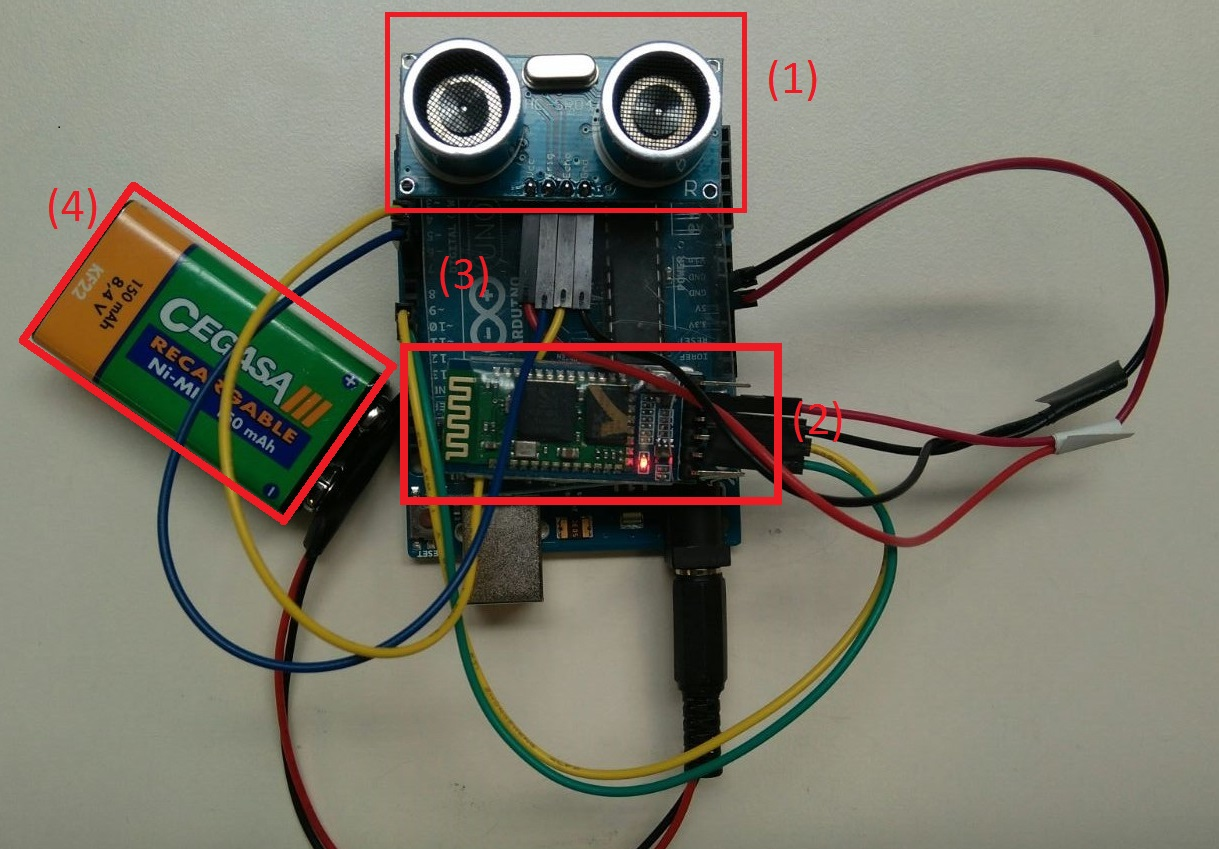
\includegraphics[width=0.7\textwidth]{./graphics/sensor}
 	\caption{Prototipo de sensor de ultrasonidos} \label{fig:sensor_ultrasonido}
 \end{figure}

	\subsubsection{Conexionado del sensor}
		El conexionado del prototipo (apartado \ref{su}), aparece representado de manera esquemática en la Figura \ref{fig:conexionado} con el fin de clarificar las conexiones. En un futuro diseño más compacto, la placa utilizada, así como algunos de los componentes, serán modificados manteniendo el enfoque de bajo coste, ergonomía y precisión. Por ello las conexiones podrán ser modificadas según sea necesario.
		
		 
		\begin{figure}[H]
			\centering
			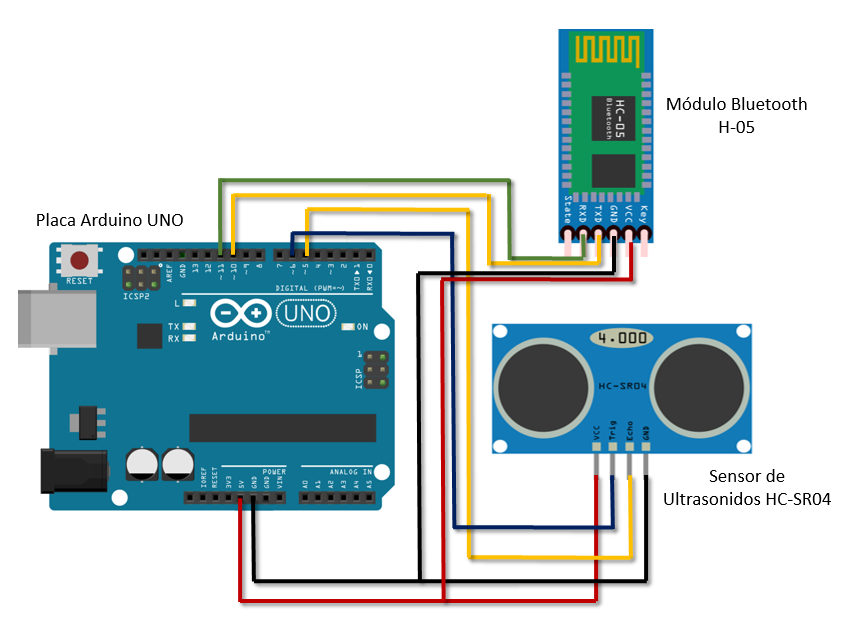
\includegraphics[width=0.7\textwidth]{./graphics/conexionado}
			\caption{Esquema de conexión del sensor de ultrasonido} \label{fig:conexionado}
		\end{figure}
		
	\subsection{Comunicación del sensor}
	
		\subsubsection{Bluetooth}
		
		Para el envío de la información de distancia desde la placa Arduino hasta el PC donde se van a procesar los datos, se ha elegido el módulo comercial Bluetooth H-05 que aparece representado en la Figura \ref{fig:bluetooth}.
		
	
			 \begin{figure}[H]
			 	\centering
			 	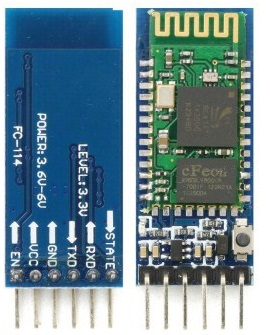
\includegraphics[width=0.25\textwidth]{./graphics/bluetooth}
			 	\caption{Módulo Bluetooth HC-05} \label{fig:bluetooth}
			 \end{figure}
			 
		Dicho módulo se comunicará con un dongle USB 4.0 en el PC ya que éste no dispone de interfaz Bluetooth de serie (ver Figura \ref{fig:dongle}). Además es compatible con estándares anteriores (2.0, 3.0) por lo que resulta apropiado para el diseño.
		
		
		\begin{figure}[H]
			\centering
			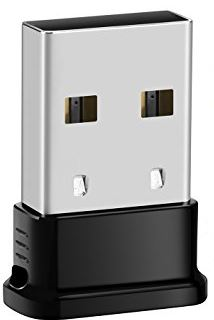
\includegraphics[width=0.15\textwidth]{./graphics/dongle}
			\caption{Dongle Bluetooth 4.0 WhiteLabel} \label{fig:dongle}
		\end{figure}
			
		\subsubsection{Software de captura}
		
		En este trabajo se ha diseñado un software de captura (Figura \ref{fig:software}) para la obtención de los datos de distancia suministrados por el sensor.
		

		Las funcionalidades principales de este software son:
		\begin{enumerate}
				\item Creación del interfaz Bluetooth para la comunicación con Matlab. 
				\item Representación de los datos recogidos en tiempo real.
				\item Posibilidad de guardar los datos en un archivo.
				\item Posibilidad de cargar un archivo y representarlo offline.
		\end{enumerate}
	
		
\section{Procedimiento de medida}		

\subsection{Set-up de medida}
Para demostrar la viabilidad del sistema en cuanto a su capacidad para medir la distancia de separación entre pasos,se proponen dos set-ups que consisten en establecer unas marcas en el suelo a una distancia conocida para así, una vez realizado el procesado de las señales, poder determinar si los resultados son correctos. El primer set-up consta de una medida de paso de 43 cm (ver Figura \ref{fig:setup_43}) y el segundo para una de 80.5 cm (ver Figura  \ref{fig:setup_80} ). 

\begin{figure}[H]
	\centering
	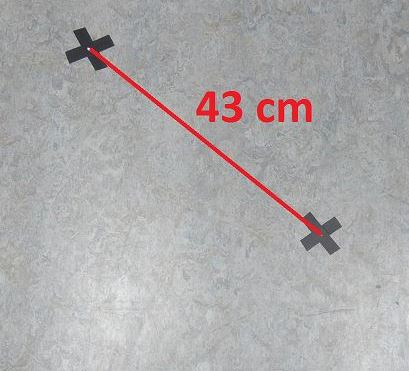
\includegraphics[width=0.55\textwidth]{./graphics/setup_43}
	\caption{Set-up de medida de un paso de 43 cm} \label{fig:setup_43}
\end{figure}

\begin{figure}[H]
		\centering
		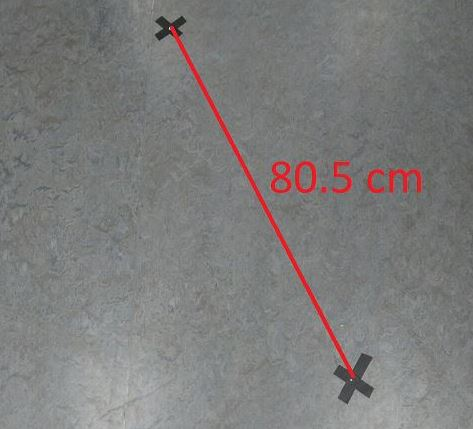
\includegraphics[width=0.55\textwidth]{./graphics/setup_80}
		\caption{Set-up de medida de un paso de 80.5 cm} \label{fig:setup_80}
\end{figure}
	
Este montaje permitirá el poder medir un la distancia de un paso para verificar que el tanto el funcionamiento como el procesado con correctos. Se dejará como línea futura el poder realizar el procesado de forma automática y para varios pasos. Para realizar las medidas se ha colocado un sensor inercial en cada pie y el sensor de ultrasonidos en el tobillo según se representa en la Figura \ref{fig:colocar} y \ref{fig:paso}. 
\begin{figure}[H]
	\centering
	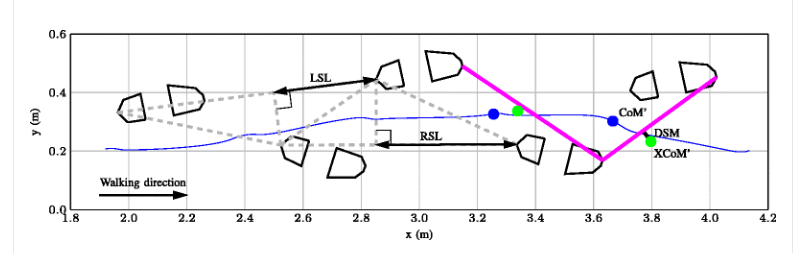
\includegraphics[width=0.55\textwidth]{./graphics/Medida}
	\caption{Colocación de los sensores para la medida} \label{fig:colocar}
\end{figure}
\begin{figure}[H]
	\centering
	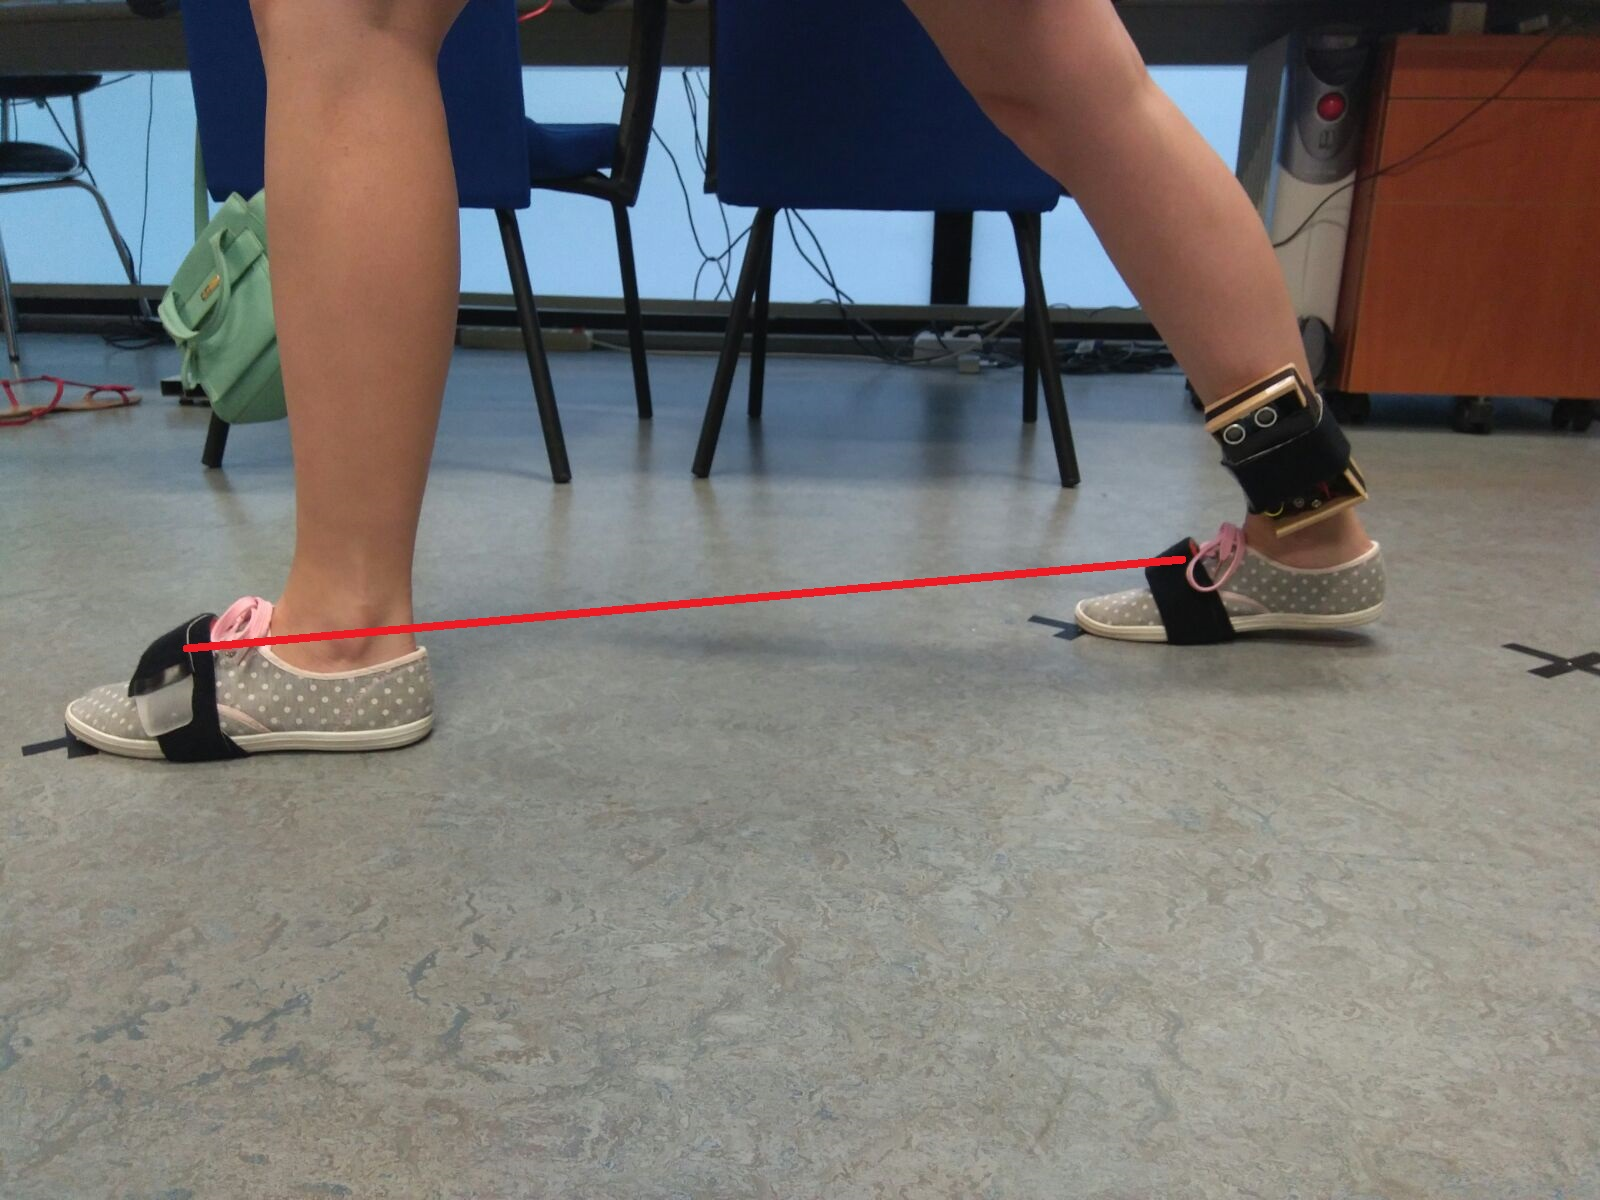
\includegraphics[width=0.65\textwidth]{./graphics/paso}
	\caption{Ejemplo de paso para la medida} \label{fig:paso}
\end{figure}


\subsection{Captura de datos}

Para llevar a cabo la medida se colocará un sensor inercial en cada pie y el sensor de ultrasonidos en uno de ellos. A continuación, se capturarán los datos de los sensores inerciales mediante el software específico MTManager de Xsens y los datos del sensor de ultrasonido mediante el software realizado con MATLAB\textsuperscript{\textregistered} 


\subsection{Sincronización}
Una de las etapas clave del diseño del sistema a tiempo real es el de la sincronización de ambos sensores. En este trabajo, para una demostración de funcionamiento, el procesado de las señales de ambos sensores se realizará por separado de forma que se pueda demostrar el funcionamiento del sistema y se dejará como línea futura de investigación la sincronización. 

Se pretende conseguir una lectura de los datos del sensor de ultrasonido en el PC con un tiempo de muestreo constante. En este punto del trabajo se encuentran dificultades con la forma en que Matlab lee los datos. Los datos enviados por el sensor son constantes pero la lectura hace ese tiempo variable. Si se consigue un tiempo constante, mediante procesados como la interpolación podría sincronizarse con los sensores inerciales. Además, debido a que se utilizan dos programas de captura, es necesario establecer un inicio que se considere como principio tanto para las señales de los sensores inerciales como el de ultrasonidos. 


\subsection{Obtención de distancia}
Para la obtención de la distancia de separación entre pasos existen tres scripts realizados con la herramienta software Matlab\textsuperscript{\textregistered}

Mediante un software en Matlab\textsuperscript{\textregistered} se cargan las señales y se realiza el post-procesado para obtener cada una de las distancias que van a permitir la obtención de la distancia de separación entre pasos.

Se procesará el cálculo de las distancias deseadas de los sensores inerciales y del de ultrasonido y dichas informaciones se utilizarán para la obtención de la distancia de separación entre pasos.

\subsubsection{Sensores inerciales}

	
	Para la obtención del dato de distancia a partir de las señales proporcionados por los sensores inerciales es necesario tener en cuenta que la distancia se recorre en el plano en el que se produce el avance, que es este caso es el plano XY.

Para obtener la posición en este plano a partir de la aceleración en los tres ejes XYZ proporcionada por los sensores inerciales, es necesaria una doble integración.Posteriormente se elimina la deriva existente en las señales debido a esta integración. A continuación se describen los cálculos realizados

\begin{itemize}
	
	\item{\textbf{Obtención de la velocidad}}
	
		Se realiza una primera integración de la aceleración en el eje X y en el eje Y de donde se obtiene la velocidad tal y como aparece en la Figura \ref{fig:vel_no_corr}
	 \begin{figure}[H]
	 	\centering
	 	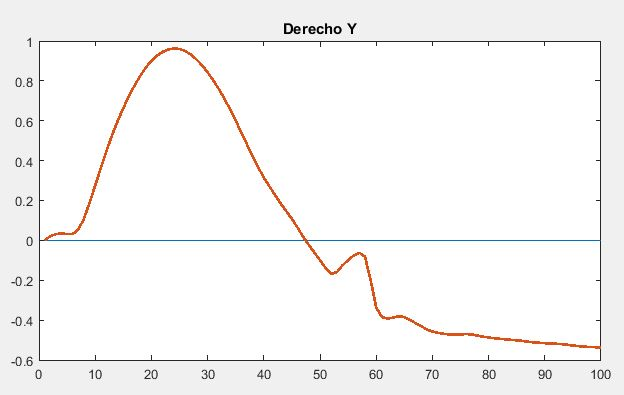
\includegraphics[width=0.81\textwidth]{./graphics/vel_no_corr}
	 	\caption{Ejemplo de deriva en la señal} \label{fig:vel_no_corr}
	 	
	 \end{figure}
 
	\item{\textbf{Obtención de la velocidad sin deriva}}	
	
En el instante de inicio y fin del paso, cuando el pie permanece apoyado, la velocidad debe ser cero.. Para lograr eliminar la deriva en la señal se propone utilizar la ecuación de la recta (color morado) que aparece en la Figura  \ref{fig:vel_no_corr_rect} . Dicha recta entre dos puntos A(a1, a2) y B(b1,b2) se difine mediante la ecuación \ref{eq:recta}
	
	\begin{equation}\label{eq:recta}
	y = (\frac{b_{2}-b_{1}}{a_{2}-a_{1}})*(x-a_{1})+b_{1}
	\end{equation}
	
	;donde:
	\begin{itemize}
		\item b2: coordenada y del último punto escogido (B)
		\item b1: coordenada x del último punto escogido (B)
		\item a2: coordenada x del primer punto escogido (A)
		\item a1: coordenada y del primer punto escogido (A)

	
	\end{itemize}


		 \begin{figure}[H]
		 	\centering
		 	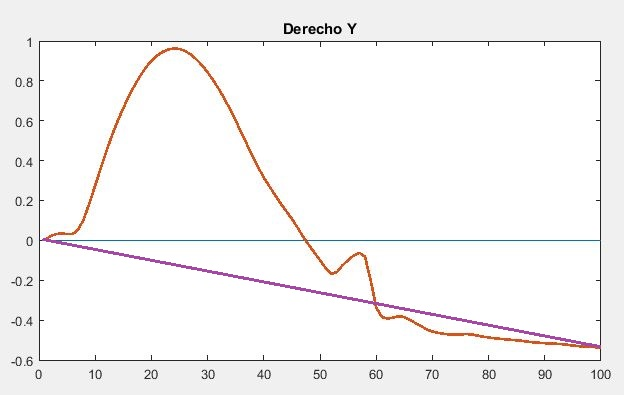
\includegraphics[width=0.8\textwidth]{./graphics/vel_no_corr_deriva}
		 	\caption{Recta para la corrección de la deriva} \label{fig:vel_no_corr_rect}
		 	
		 \end{figure}
De esta forma restando a la señal de velocidad la recta calculada, el resultado es el que aparece en la Figura \ref{fig:corregida} donde se representa la velocidad sin deriva.

	
		 \begin{figure}[H]
		 	\centering
		 	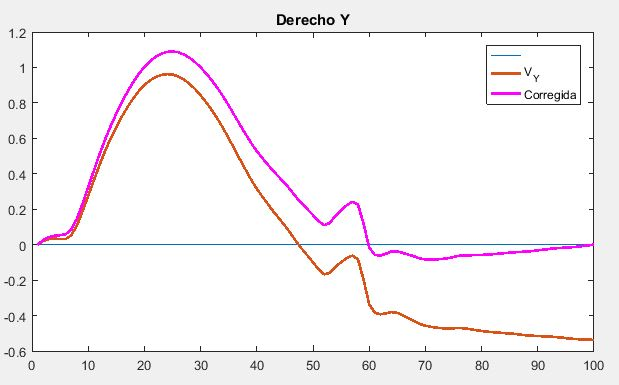
\includegraphics[width=0.8\textwidth]{./graphics/corregida}
		 	\caption{Ejemplo eliminación de la deriva} \label{fig:corregida}
		 \end{figure}


	\item{\textbf{Obtención de distancia D2 de sensores inerciales}}

	
	Una vez corregida la deriva en las velocidades X e Y de los sensores izquierdo y derecho en necesaria una segunda integración para hallar la posición en cada uno de los ejes. A continuación se representa la posición en el eje X con respecto al eje Y para calcular la distancia total en el plano XY (ver Figura \ref{fig:posi})
	\begin{figure}[H]
		\centering
		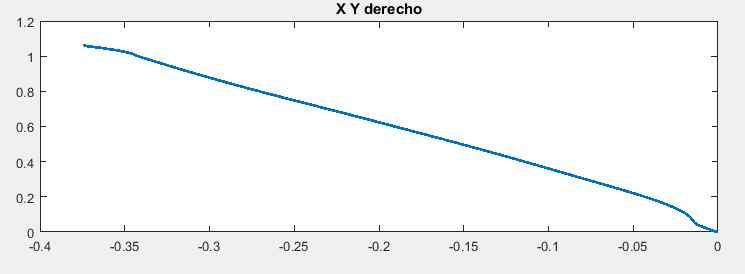
\includegraphics[width=1\textwidth]{./graphics/posi}
		\caption{Ejemplo eliminación de la deriva} \label{fig:posi}
		
	\end{figure}
	
	Para el cálculo de la distancia será necesario la eliminación de la deriva en la posición.
	
	La distancia (D2) ahora será la distancia entre los puntos inicial y final de la Figura \ref{fig:posi}, una vez corregida la deriva, que se calculará mediante la ecuación \ref{eq:pos}
		\begin{equation}\label{eq:pos}
		Distancia = \sqrt{(b_{1}-a_{1})^{2}+(b_{2}-a_{2})^{2}}
		\end{equation}
		\begin{equation}\label{eq:punto2}
			B = [b_{1},b_{2}]	
		\end{equation}
		\begin{equation}\label{eq:puntos1}
			A = [a_{1},a_{2}]
		\end{equation}
		;donde:
		\begin{itemize}
		\item b2: coordenada y del último punto escogido (B)
		\item b1: coordenada x del último punto escogido (B)
		\item a2: coordenada x del primer punto escogido (A)
		\item a1: coordenada y del primer punto escogido (A)
		\end{itemize}
\end{itemize}



\subsubsection{Sensor de ultrasonido}

	Previamente a la obtención de la distancia que se desea obtener usando el sensor de ultrasonido, se realiza una comprobación del correcto funcionamiento tanto del dispositivo como del envío de datos al PC vía Bluetooth. Inicialmente se realizan medidas con el sensor en estático. Para ello se propone el set-up de medida que aparece representado en la Figura  \ref{fig:ultrasonido}.
		
		 \begin{figure}[H]
		 	\centering
		 	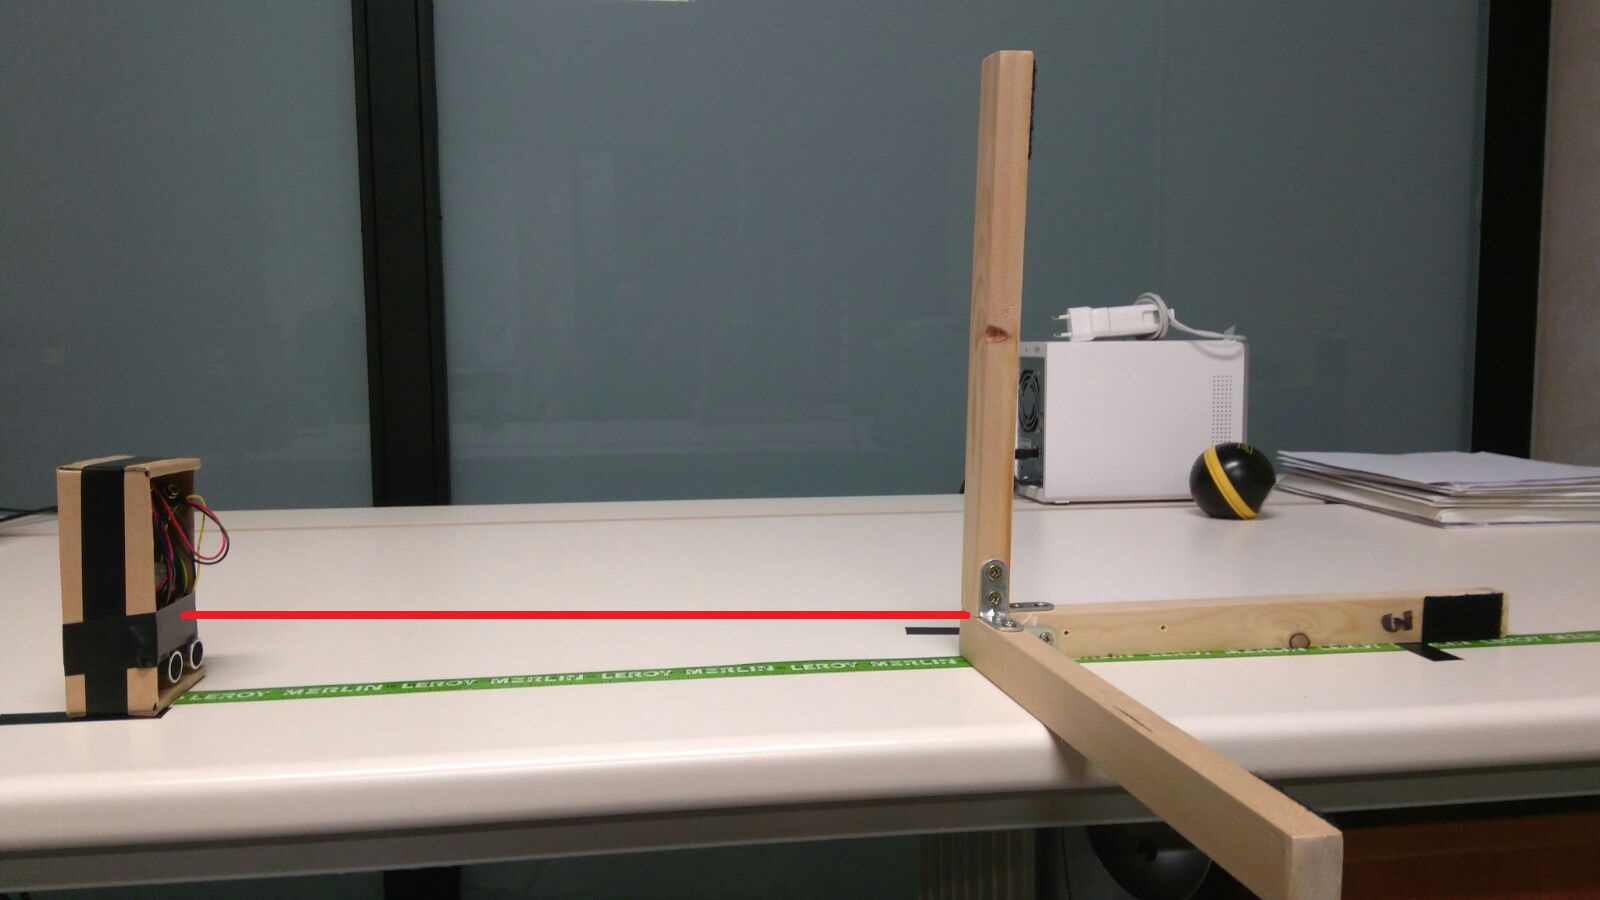
\includegraphics[width=0.95\textwidth]{./graphics/ultrasonido}
		 	\caption{Setup medida estática de sensor de ultrasonido}\label{fig:ultrasonido}
		 \end{figure}

Para estimar la precisión y el correcto funcionamiento del sensor se ha calculado el error absoluto y relativo de cada una de las medidas realizadas.

Una vez hecha dicha comprobación en estático, se añade al sistema de medida completo. Para ello se coloca el sensor en el tobillo y con el sensor orientado hacia la otra pierna (ver Figura \ref{fig:ultracoloc}).
		
	 \begin{figure}[H]
	 	\centering
	 	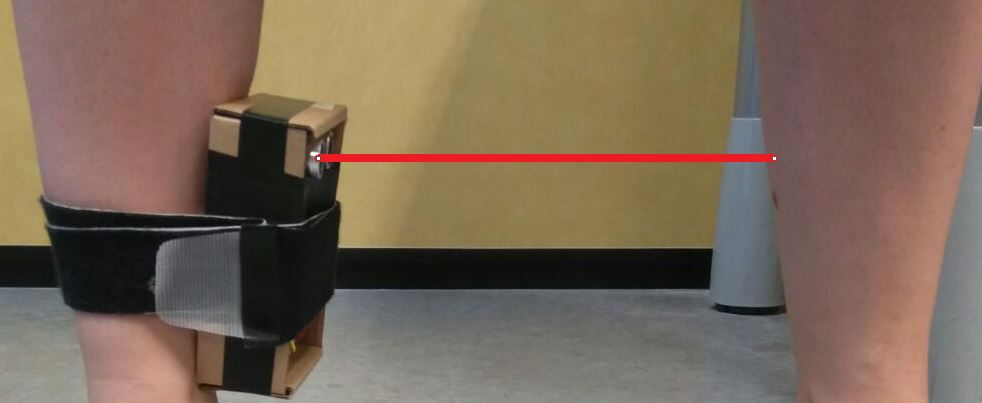
\includegraphics[width=0.8\textwidth]{./graphics/coloc_ultr}
	 	\caption{Colocación de sensor para medidas en dinámico} \label{fig:ultracoloc}
	 \end{figure}
				
		
\subsubsection{Obtención de distancia de separación entre pasos}

Una vez calculadas las distancias necesarias, se procede al cálculo de la distancia de separación entre pasos. En la Figura \ref{fig:sep} se representa dicho cálculo. La distancia D2 es la correspondiente al cálculo de la distancia con el sensor inercial izquierdo en este caso, la distancia D1 es la distancia calculada mediante el sensor de ultrasonido.
\begin{figure}[H]
	\centering
	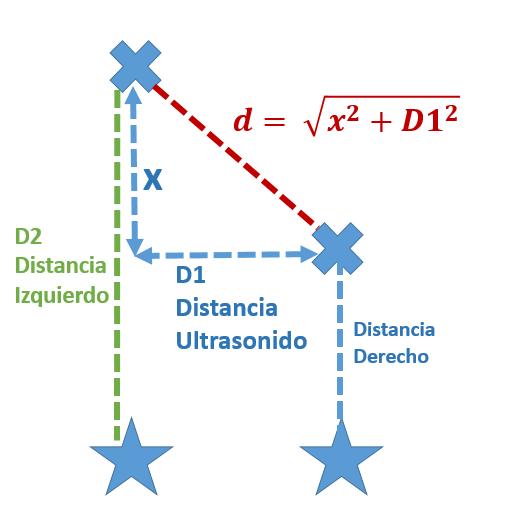
\includegraphics[width=0.8\textwidth]{./graphics/sep}
	\caption{Cálculo final de distancia de separación entre pasos} \label{fig:sep}
\end{figure}

Por tanto, para obtener X se utiliza la ecuación \ref{eq:x}
\begin{equation}\label{eq:x}
x = D2 - DistanciaDerecho
\end{equation}
En el caso de que el primero de los pasos se comenzase con el izquierdo la ecuación es la relativa a la DistanciaIzquierdo.

Para determinar la distancia, se utiliza por tanto, la ecuación \ref{eq:d}
\begin{equation}\label{eq:d}
d = \sqrt{x^{2}+D1^{2}}
\end{equation}
\thispagestyle{empty}

%
% Resultados
%
\chapter{Resultados y análisis\label{sec:resultados}}

\section{Resultados en estático}

\section{Resultados en movimiento}

\section{Resultados en pacientes}

\afterpage{\blankpage}
\thispagestyle{empty}

%
% Conclusiones
%
\chapter{Conclusiones y líneas futuras\label{sec:conclusiones}}


%Este ejercicio resulta verdaderamente beneficioso en el aprendizaje. 


Los resultados de este trabajo han sido útiles para determinar la viabilidad al realizar un primer prototipo como solución al problema planteado. El comparar dos tecnologías diferentes para una misma aplicación permite entender en mayor magnitud las posibilidades de cada una de las tecnologías. 


%Este ha sido un trabajo muy completo al tomar tanto en cuenta ejercicio de desarrollo software como hardware. 

Durante la realización del prototipo basado en redes de difracción de Bragg se han encontrado diversas dificultades:

\begin{itemize}
	\item \textbf{Tecnología muy delicada.} La fibra del sensor FBG es muy delicada para el proceso de fabricación del guante y las herramientas disponibles en el laboratorio. 
	Tanto en el proceso de fabricación como en la posterior manipulación la fragilidad de las fibras hace prácticamente imposible su futuro uso como sensor de movimiento para esta aplicación.
	%Pese haber tenido mucho cuidado a la hora de manipularla ha sido imposible evitar que se rompiera en múltiples ocasiones. Además una vez el prototipo ha sido fabricado con éxito, sin que se rompa ninguna fibra, estas siguen siendo susceptibles de romperse. Por ello no es la mejor tecnología para medir movimientos continuados, que rompen la fibra pese a estar embebida en PDMS. 
	 
	\item \textbf{Diseño del guante no apto para todas las manos.} El diseño del guante no es apropiado para la finalidad inicial del prototito. %Al no ser posible colocar siempre el guante en la misma posición sobre la mano, las medidas obtenidas de una misma posición en diferentes ocasiones son diferentes. Mucho más aún cuando se colocan en manos con diferente fisionomía. 
	%, lo que dificulta la caracterización del movimiento respecto al comportamiento de los sensores. 
	Se trata de un condicionamiento importante. Para conseguir caracterizar el comportamiento de las FBGs con los ángulos de apertura es necesario que siempre se coloque el guante de tal forma que el vértice del ángulo coincida en el mismo punto. La forma de las diferentes manos de las personas hace que no sea posible una caracterización como la citada. Unicamente puede ser útil para evaluar el rango de movimiento y velocidad dentro de una misma sesión de rehabilitación. Aunque se pierda la información frente a una referencia global del movimiento, sigue ofreciendo al usuario una experiencia satisfactoria pese a no cumplir con la plenitud de los objetivos marcados.
	
	Para medir en cualquier tipo de mano con una referencia global, el diseño sería mucho más complejo. Haría falta buscar la manera de se pudiera colocar cada dedo independientemente para ajustar la posición del vértice del ángulo a medir y reforzar el recubrimiento de los sensores impidiendo que se dieran las deformaciones que la fibra no sea capaz de soportar.
	
	
	
	\item \textbf{Software no escalable.} Pese a ser LabVIEW un lenguaje cuya programación es muy visual, cuando se trata de partir de un proyecto desarrollado, como es el caso del software del interrrogador, resulta bastante tedioso adaptar el nuevo programa.
	
	Además la experiencia de usuario se ve muy limitada ya que LabVIEW no es muy configurable en la parte de front-end.
	
	Otro contratiempo importante del software son los problemas que da al iniciarlo. Al iniciar el software del interrogador saltan alertas de error en la señal que no permiten seguir con la ejecución. Durante el desarrollo del proyecto se ha conseguido intuir el procedimiento en el que dichas alertas saltan con menos frecuencia y de ello surgen ciertos pasos del protocolo de medida.  %-viene de fbg- 
	 
	
	 
\end{itemize}

\clearpage

Se concluye el trabajo descartando la tecnología de sensores de FBG para la evaluación de la rehabilitación de las manos. Siendo esto motivado por no cumplir con las expectativas funcionales requeridas, además de por la complejidad de su manufacturación y su delicadeza. 

Se ha propuesto un diseño que cumplirá con las expectativas de medir el movimiento de las manos, obteniendo datos comparables entre sesiones. La solución planteada presta especial atención las especificaciones que el prototipo de FBG no ha cumplido. Ofrecerá mayor versatilidad y capacidad para añadir nuevas funcionalidades. Los sensores inerciales permitirán comunicación inalámbrica, robustez del diseño y bajo precio.








\section{Líneas futuras}

A partir de la experiencia del desarrollo de este proyecto se realizará el guante basado en sensores inerciales propuesto en la memoria.

\begin{itemize}
	\item El desarrollo del guante sensorizado se realizará siguiendo un proceso modular. Se dividirá el escenario global en varios escenarios, simplificando así su realización. Añadiendo las funcionalidades de cada dedo progresivamente, comenzando por el pulgar y el índice. 
	 
	\item En paralelo a este desarrollo se realizará el desarrollo del software por su dependencia, dejando para el final el desarrollo grueso de las funcionalidades más allá de la interpretación de las medidas de los sensores. 
	
	%La aplicación se programará en C++, siendo más adaptable a las necesidades de programación. Así el desarrollador tiene más facultad a la hora de programar. 
	 
	\item La aplicación se programará en C++, debido a que tiene una extensa documentación y es mas moldeable segun nuestras necesidades.
	
	\item Debido al contexto en el que se aplica el sistema, se debe tener en cuenta la ergonomía del mismo, la autonomía y el coste.
	Asimismo deberá cumplir con unas especificaciones óptimas para poder obtener resultados fiables. Sería recomendable contar con la experiencia de in ingeniero de diseño que paralelamente, con el desarrollo electrónico, procesado de señal y comunicaciones, se centre en el ámbito del diseño y la ergonomía del dispositivo.
	
	
	%Este diseño tiene capacidad para abarcar más funcionalidades de las propuestas. El desarrollo de estas no corresponde a esta memoria, pero merecen mención en este apartado para comprender mejor el alcance de esta tecnología. 
	
	\item El guante contará con capacidad inalámbrica, haciendo su uso mucho más cómodo al aportarle portabilidad.
	
	\item Una posibilidad más que ofrece el guante es añadirle funcionalidad actuadora para acompañar a los pacientes en el movimiento de las manos durante sus ejercicios de rehabilitación. 
\end{itemize} 

%
% Página en blanco
%
\afterpage{\blankpage}
\thispagestyle{empty}
%
% Bibliografía
%
\printbibliography[heading=bibintoc]

% No expandir elementos para llenar toda la página
\raggedbottom

%
% Apéndices
%
%\appendix
%\cleardoublepage
%\addappheadtotoc
%\appendixpage
\newpage\null\thispagestyle{empty}
%
% TODO: Apéndices del TFM
%
%\chapter{Algoritmos empleados\label{sec:ejemplos}}

%
% Breve guía de comandos útiles para la memoria
%



% Citar un elemento del glosario
Citamos el acrónimo \gls{FPGA}.

% Citar un elemento del glosario (primera letra en may´usculas)
\Gls{bitstream} es una secuencia de bits.

% Insertar una imagen con pie de página
\begin{figure}[H]
  \centering
  
\includegraphics[width=0.14\textwidth,clip=true]{escudo}
  \caption{Logo de la Universidad Pública de Navarra.}
  \label{fig:logo_upna}
\end{figure} 

% Referenciar una etiqueta (label)
La figura~\ref{fig:logo_upna} se utiliza en la portada.

% Nueva página
\clearpage



% Fórmula dentro de una línea de texto
La ecuación de Euler ($e^{ \pm i\theta } = \cos \theta \pm i\sin \theta$) es citada frecuentemente como un ejemplo de belleza matemática.

% Fórmula independiente
\begin{equation}\label{eq:pythagoras}
a^2 + b^2 = c^2
\end{equation}


	
\section{Arduino}
	
		% Añadir código fuente sin líneas
		\begin{lstlisting}[label=algoritmo:Arduino,language=C,frame=single,caption=Algortimo en Arduino para obtención de distancia sensor ultrasonido]
	#include <SoftwareSerial.h> 
			
	SoftwareSerial BT(10,11);
			
	const int EchoPin = 5;
	const int TriggerPin = 6;
			
	void setup() {
		BT.begin(9600);
		pinMode(TriggerPin, OUTPUT);
		pinMode(EchoPin, INPUT);
	}	
	void loop() {
		int cm = ping(TriggerPin, EchoPin);
		BT.println(cm);
		delay(60);
	}
			
	int ping(int TriggerPin, int EchoPin) {
		long  distancia;
		long duration;
		digitalWrite(TriggerPin, LOW);  
		delayMicroseconds(4);
		digitalWrite(TriggerPin, HIGH); 
		delayMicroseconds(10);
		digitalWrite(TriggerPin, LOW);		
		duration = pulseIn(EchoPin, HIGH);  	
		distancia = duration * 10 / 292 / 2;  
		return distancia;			
}
		\end{lstlisting}
	

% Fin del documento
\end{document}
